\documentclass[]{../tex/krantz}
\usepackage[spanish]{babel}
\usepackage[utf8]{inputenc}
\DeclareUnicodeCharacter{200B}{{\hskip 0pt}}
\input{../tex/pdf-settings}
\input{../tex/es-settings}

\begin{document}

\title{Enseñar tecnología en comunidad}
\subtitle{Cómo crear y dar lecciones que funcionen \\ y construir una comunidad docente a su alrededor}
\author{Greg Wilson}
\date{Taylor \& Francis, 2019, 978-0-367-35328-5}
\maketitle

\frontmatter
\dedication{
Para mi madre, Doris Wilson,\\
que enseñó a cientos de niñas y niños a leer y creer en sí mismas/os.\\
~\\
Y para mi hermano Jeff, que no vivió para verlo terminado.\\
``Recuerda, todavía tienes muchos momentos buenos frente a ti.''\\
~\\
~\\
La traducción de este libro está dedicada a la memoria de \hreffoot{https://es.wikipedia.org/wiki/Rebeca_Guber}{Rebeca Cherep de Guber}
~\\
~\\
Todas las regalías de la venta de la versión en español de este libro se donan a\\
\hreffoot{https://www.metadocencia.org/}{MetaDocencia},\\
una organización basada en trabajo voluntario que enseña\\
a docentes de habla hispana de todo el mundo
a enseñar de forma efectiva usando prácticas basadas\\
en evidencia .
}


\tableofcontents
\include{rules}
\chapter*{Sobre la traducción}\label{s:traduccion}

Este es el sitio web de la versión en español, \textbf{aún en proceso de traducción}, de \emph{Teaching Tech Together} de Greg Wilson.
La traducción de \emph{Enseñar Tecnología en Comunidad} es un proyecto colaborativo
de voluntarias de la comunidad de \hreffoot{https://www.metadocencia.org/}{MetaDocencia} y 
\hreffoot{https://rladies.org/}{R-Ladies} en Latinoamérica,
que tiene por objetivo traducir al español material actualizado 
y de calidad para hacerlo accesible a hispanohablantes.
Iniciamos la traducción en Marzo del año 2020 y esta actualización corresponde a Marzo de 2021.

El trabajo se organizó de manera que cada capítulo tuvo una persona asignada a cargo de la traducción 
y dos personas que realizaron las revisiones de cada capítulo.  
Se buscó que el idioma de las traductoras y revisoras tuviera origen en diferentes países para
poder considerar las diferentes y hermosas formas en que hablamos español en todo el mundo.
Al finalizar todo el proceso se realizó una edición final de todo el libro en su conjunto.

Tomamos algunas decisiones para el proceso de traducción basado en experiencias previas
del equipo y otras guías de traducciones colaborativas al español como 
\hreffoot{https://github.com/cienciadedatos/documentacion-traduccion-r4ds}{R para Ciencia de Datos}
y \hreffoot{https://github.com/Carpentries-ES/board/blob/master/Convenciones\_Traduccion.md}{\emph{The Carpentries}}:

La variedad dialéctica del español (castellano) utilizada en la traducción corresponde 
a Latinoamérica y se utilizó una voz conversacional en lugar de una voz formal o académica.

Decidimos intentar ajustar la redacción para evitar la marca de género, pero
en caso de no poder evitar su uso, decidimos utilizar lenguaje no sexista  
que implica el uso del femenino y masculino privilegiando la agilidad y fluidez del texto, 
que el mismo se entienda y que sea claro el mensaje. Para que haya coherencia 
a lo largo del texto y mostrar que no hay una determinada jerarquía 
alternamos el uso del femenino/masculino o masculino/femenino entre capítulos 
y el uso fue consistente durante todo el capítulo. 

También decidimos buscar las versiones al español de referencias como 
entradas en \emph{Wikipedia} y lecciones de \emph{The Carpentries}.  En caso que no existieran 
se dejaron las versiones en inglés.

Finalmente, se decidió cambiar algunos ejemplos a realidades más regionales, 
para que sean más cercanos a la región de donde son la mayoría de las
traductoras.

Quienes trabajamos en este proyecto somos (en orden alfabético):
\hreffoot{https://twitter.com/\_lacion\_}{Laura Acion},
\hreffoot{https://twitter.com/MonicaLA2000}{Mónica Alonso},
\hreffoot{https://twitter.com/Zjbb}{Zulemma Bazurto},
\hreffoot{https://twitter.com/AlejaBellini}{Alejandra Bellini},
\hreffoot{https://twitter.com/yabellini}{Yanina Bellini Saibene},
\hreffoot{https://twitter.com/July\_Benitezs}{Juliana Benitez Saldivar},
\hreffoot{https://twitter.com/luucamay\_}{Lupe Canaviri Maydana},
\hreffoot{https://twitter.com/spcanelon}{Silvia Canelón},
\hreffoot{https://twitter.com/ruthy\_root}{Ruth Chirinos},
\hreffoot{https://twitter.com/PaobCorrales}{Paola Corrales},
\hreffoot{https://twitter.com/DermitMaria}{María Dermit},
\hreffoot{https://twitter.com/anadiedrichs}{Ana Laura Diedrich},
\hreffoot{https://twitter.com/patriloto}{Patricia Loto},
\hreffoot{https://twitter.com/pmnatural}{Priscilla Minotti},
\hreffoot{https://twitter.com/Nat\_Mora\_}{Natalia Morandeira},
\hreffoot{https://twitter.com/\_luciarp\_}{Lucía Rodríguez Planes},
\hreffoot{https://twitter.com/palolili23}{Paloma Rojas},
\hreffoot{https://twitter.com/YkSosaP}{Yuriko Sosa}
\hreffoot{https://www.linkedin.com/in/natalie-stroud-63110a113/}{Natalie Stroud},
y \hreffoot{https://twitter.com/\_yarena}{Yara Terrazas-Carafa}.

En cada capítulo encontrarás el detalle de las personas que estuvieron a cargo de traducirlo
y revisarlo.

La coordinación del trabajo estuvo a cargo de Yanina Bellini Saibene y 
la edición final a cargo de Yanina Bellini Saibene y Natalia Morandeira.

\hreffoot{https://www.instagram.com/malenazabalegui/}{Malena Zabalegui} nos aconsejó sobre el uso de lenguaje no sexista e 
inclusivo para la realización de esta traducción y \hreffoot{https://www.instagram.com/fetch.franciscoetchart/}{Francisco Etchart}
diseñó el hex sticker.

También generamos un
\hreffoot{https://yabellini.shinyapps.io/T3Glossary/}{glosario y 
diccionario bilingüe de términos de educación y tecnología}
a partir del glosario del libro y del listado de términos 
a traducir (o no) del libro.
El desarrollo de este glosario estuvo a cargo de Yanina Bellini Saibene utilizando
\hreffoot{https://carpentries.github.io/glosario/}{glosario}.

Todos los detalles del proceso de traducción se pueden consultar
\hreffoot{https://github.com/gvwilson/teachtogether.tech/blob/master/es/README.md}{en la documentación del proyecto}.


\mainmatter
\chapter{Introduction}\label{s:intro}

Hundreds of grassroots groups have sprung up around the world to teach
programming, web design, robotics, and other skills to
\glossref{g:free-range-learner}{free-range learners} outside
traditional classrooms.  These groups exist so that people don't have
to learn these things on their own, but ironically, their founders and
instructors are often teaching themselves how to teach.

There's a better way. Just as knowing a few basic facts about germs
and nutrition can help you stay healthy, knowing a few things about
psychology, instructional design, inclusivity, and community
organization can help you be a more effective teacher. This book
presents evidence-based practices you can use right now, explains why
we believe they are true, and points you at other resources that will
help you go further.  Its four sections cover:

\begin{itemize}

\item
  how people learn;

\item
  how to design lessons that work;

\item
  how to deliver those lessons; and

\item
  how to grow a community of practice around teaching.

\end{itemize}

\noindent
Throughout, we try to follow our own advice: for example, we start
with ideas that are short, engaging, and actionable in order to
motivate you to read further (\chapref{s:motivation}), include lots of
exercises that can be used to reinforce learning (\chapref{s:models}),
and include the original design for this book in \appref{s:v3} so that
you can see what a lesson design looks like.

\begin{callout}{This Book Belongs to Everyone}

  This book is a community resource.  Parts of it were originally
  created for
  \href{http://carpentries.github.io/instructor-training/}{the
    Software Carpentry instructor training program}, which has been
  run over several hundred times over the past six years, and all of
  it can be freely distributed and re-used under the
  \href{https://creativecommons.org/licenses/by/4.0/}{Creative Commons
    - Attribution 4.0 license}.  Please see {\website} to download a
  digital version or to purchase a printed copy at cost.

  Contributions of all kinds are welcome, from errata and minor
  improvements to entirely new sections and chapters.  All proposed
  contributions will be managed in the same way as edits to Wikipedia
  or patches to open source software, and all contributors will be
  credited for their work each time a new version is released.  Please
  see \appref{s:joining} for details and \secref{s:joining-covenant}
  for our code of conduct.

\end{callout}

\section{Who You Are}\label{s:intro-audience}

\secref{s:process-personas} explains how to figure out who your
learners are.  The four I had in mind when writing this book are all
\glossref{g:end-user-teacher}{end-user teachers}: teaching isn't their
primary occupation, they have little or no background in pedagogy, and
they may work outside institutional classrooms.

\begin{description}

  \item[Emily] trained as a librarian, and now works as a web designer
    and project manager in a small consulting company.  In her spare
    time, she helps run web design classes for women entering tech as
    a second career.  She is now recruiting colleagues to run more
    classes in her area using the lessons that she has created, and
    wants to know how to grow a volunteer teaching organization.

  \item[Moshe] is a professional programmer with two teenage children
    whose school doesn't offer programming classes.  He has
    volunteered to run a monthly after-school programming club, and
    while he frequently gives presentations to colleagues, he has no
    experience designing lessons.  He wants to learn how to build
    effective lessons in collaboration with others, and is interested
    in turning his lessons into a self-paced online course.

  \item[Samira] is an undergraduate in robotics who is thinking about
    becoming a full-time teacher after she graduates.  She wants to
    help teach weekend workshops for undergraduate women, but has
    never taught an entire class before, and feels uncomfortable
    teaching things that she's not an expert in.  She wants to learn
    more about education in general in order to decide if it's for
    her.

  \item[Gene] is a professor of computer science whose research area
    is operating systems.  They have been teaching undergraduate
    classes for six years, and increasingly believe that there has to
    be a better way. The only training available through their
    university's teaching and learning center relates to posting
    assignments and grades in the learning management system, so they
    want to find out what else they ought to be asking for.

\end{description}

\noindent
These people have \emph{a variety of technical backgrounds} and
\emph{some previous teaching experience}, but \emph{no formal training
  in teaching, lesson design, or community organization}.  Most work
with \emph{free-range learners} and are \emph{focused on teenagers and
  adults} rather than children; all \emph{have limited time and
  resources}.

\secref{s:joining-using} describes different ways people have used
this material.  (That discussion is delayed to an appendix because it
refers to some of the ideas introduced later in this book.)  We expect
our made-up learners to use this material as follows:

\begin{description}

  \item[Emily] will take part in a weekly online reading group with
    her volunteers.

  \item[Moshe] will cover part of this book in a two-day weekend
    workshop and study the rest on his own.

  \item[Samira] will use this book in a one-semester undergraduate
    course with assignments, a project, and a final exam.

  \item[Gene] will read the book on their own in their office or
    while commuting, wishing all the while that universities did more
    to support high-quality teaching.

\end{description}

\section{What to Read Instead}\label{s:intro-instead}

If you are in a hurry, or want a taste of what this book will cover,
\cite{Brow2018} presents ten evidence-based tips for teaching
computing.  You can download the paper, or read it online, on
\href{https://doi.org/10.1371/journal.pcbi.1006023}{the PLoS website}.

I also recommend:

\begin{itemize}

  \item \href{http://carpentries.github.io/instructor-training/}{The
    Carpentries instructor training}, for which most of the first half
    of this book was originally developed.

  \item \cite{Lang2016} and \cite{Hust2012}, which are short,
    approachable, and connect things you can do right now to the
    research that backs them.

  \item \cite{Majo2015}, \cite{Broo2016} \cite{Berg2012}, and
    \cite{Rice2018}.  The first catalogs a hundred different kinds of
    exercises you can do with students; the second describes fifty
    different ways that groups can discuss things productively, while
    the third is a collection of patterns for teaching, and the fourth
    explains why to give learners breaks in class and ways to use them
    productively.  These books can be used on their own, but I think
    they make more sense once Huston or Lang have given you a
    framework for understanding them.

  \item \cite{DeBr2015}, which conveys a lot of what \emph{is} true
    about educational by explaining what \emph{isn't}, and
    \cite{Dida2016}, which grounds learning theory in cognitive
    psychology.

  \item \cite{Pape1993}, which remains an inspiring vision of how
    computers could change education.

  \item \cite{Gree2014}, \cite{McMi2017} and \cite{Watt2014}.  These
    three short books explain why so many attempts at educational
    reform have failed over the past forty years, how for-profit
    colleges are exploiting and exacerbating the growing inequality in
    our society, and how technology has repeatedly failed to
    revolutionize education.

  \item \cite{Guzd2015a}, \cite{Hazz2014}, and \cite{Sent2018}, which
    are academically-oriented books I've found about teaching
    computing.

  \item \cite{Brow2007} and \cite{Mann2015}, because you can't teach
    computing well without changing the system in which we teach, and
    you can't do that on your own.

\end{itemize}

Of these, \cite{Pape1993} is the one that shaped my ideas about
teaching the most.  Papert's central argument is that people don't
absorb knowledge; instead, they (re-)construct it for themselves, and
computers are a new and powerful tool for helping them do that.
\href{https://medium.com/bits-and-behavior/mindstorms-what-did-papert-argue-and-what-does-it-mean-for-learning-and-education-c8324b58aca4}{Andy
  Ko's excellent description} does a better job of summarizing
Papert's ideas than I possibly could, and \cite{Craw2010} is a
thought-provoking companion to both.

\section{History}\label{s:intro-history}

\emph{A lot of my stories aren't true, but this is a true
  story{\ldots}}

When I started teaching people how to program in the late 1980s, I
went too fast, used too much jargon, and had no idea how much my
learners actually understood.  I got better over time, but still felt
like I was stumbling around in a darkened room.

In 2010, I rebooted a project called
\href{http://carpentries.org}{Software Carpentry} that teaches basic
computing skills to researchers.  (The name ``carpentry'' was chosen
to distinguish what we taught from software engineering: we were
trying to show people the digital equivalent of painting a bathroom,
not building the Channel Tunnel.)  In the years that followed, I
discovered resources like \href{http://computinged.wordpress.com}{Mark
  Guzdial's blog} and the book \emph{How Learning Works}
\cite{Ambr2010}. These in turn led me to books like
\cite{Hust2012,Lemo2014,Lang2016} that showed me how to build and
deliver better lessons in less time and with less effort.

I started using these ideas in \href{http://carpentries.org}{Software
  Carpentry} in 2012.  The results were everything I'd hoped for, so I
began running training sessions to pass on what I'd learned.  Those
sessions became a
\href{https://carpentries.github.io/instructor-training/}{training
  program} that dozens of trainers have now taught to over a thousand
people on six continents.  Since then, I have run the course for
people who teach programming to children, librarians, and women
re-entering the workforce or changing careers, and all of those
experiences have gone into this book.

\section{Why Learn to Program?}\label{s:intro-why}

Politicians, business leaders, and educators often say that people
should learn to program because the jobs of the future will require
it; for example, \cite{Scaf2017} found that people who aren't software
developers but who still program make higher wages than comparable
workers who do not.

However, as Benjamin Doxtdator has
\href{http://www.longviewoneducation.org/field-guide-jobs-dont-exist-yet/}{pointed
  out}, many of those claims are built on shaky ground.  Even if they
were true, education shouldn't prepare people for the jobs of the
future: it should give them the power to decide what kinds of jobs
there are, and to ensure that those jobs are worth doing.  And as
\href{https://computinged.wordpress.com/2017/10/18/why-should-we-teach-programming-hint-its-not-to-learn-problem-solving/}{Mark
  Guzdial points out}, there are actually many reasons to learn how to
program:

\begin{enumerate}

\item
  To understand our world.

\item
  To study and understand processes.

\item
  To be able to ask questions about the influences on their lives.

\item
  To use an important new form of literacy.

\item
  To have a new way to learn art, music, science, and mathematics.

\item
  As a job skill.

\item
  To use computers better.

\item
  As a medium in which to learn problem-solving.

\end{enumerate}

\noindent
Part of what motivates me to teach is the hope that if enough people
understand how to make technology work for them, we will be able to
build a society in which \emph{all} of the reasons above are valued
and rewarded (\chapref{s:final}).

\section{Have a Code of Conduct}\label{s:intro-code-of-conduct}

The most important thing I've learned about teaching in the last
thirty years is how important it is for everyone to treat everyone
else with respect, both in and out of class.  If you use this material
in any way, please adopt a Code of Conduct like the one in
\appref{s:conduct} and require everyone who takes part in your classes
to abide by it.

A Code of Conduct can't stop people from being offensive, any more
than laws against theft stop people from stealing.  What it \emph{can}
do is make expectations and consequences clear.  More importantly,
having one tells people that there are rules, and that they can expect
a friendly learning experience.

If someone challenges you about having a Code of Conduct, remind them
that it \emph{isn't} an infringement of free speech.  People have a
right to say what they think, but that doesn't mean they have a right
to say it wherever and whenever they want.  If they want to make
someone feel unwelcome, they can go and find their own space in which
to do it.

\section{Acknowledgments}\label{s:intro-acknowledgments}

This book would not exist without the hard work and feedback of Erin
Becker, Azalee Bostroem, Hugo Bowne-Anderson, Neil Brown, Gerard
Capes, Francis Castro, Warren Code, Ben Cotton, Richie Cotton, Karen
Cranston, Katie Cunningham, Natasha Danas, Matt Davis, Neal Davis,
Mark Degani, Michael Deutsch, Brian Dillingham, Kathi Fisler, Auriel
Fournier, Bob Freeman, Nathan Garrett, Mark Guzdial, Rayna Harris,
Ahmed Hasan, Ian Hawke, Felienne Hermans, Kate Hertweck, Toby Hodges,
Dan Katz, Christina Koch, Shriram Krishnamurthi, Katrin Leinweber,
Colleen Lewis, Lenny Markus, Sue McClatchy, Jessica McKellar, Ian
Milligan, Lex Nederbragt, Aleksandra Nenadic, Jeramia Ory, Joel
Ostblom, Elizabeth Patitsas, Aleksandra Pawlik, Sorawee
Porncharoenwase, Emily Porta, Alex Pounds, Thomas Price, Danielle
Quinn, Ian Ragsdale, Erin Robinson, Rosario Robinson, Ariel Rokem, Pat
Schloss, Malvika Sharan, Florian Shkurti, Juha Sorva, Tracy Teal,
Tiffany Timbers, Richard Tomsett, Preston Tunnell Wilson, Matt Turk,
Fiona Tweedie, Allegra Via, Anelda van der Walt, St\'{e}fan van der
Walt, Belinda Weaver, Hadley Wickham, Jason Williams, Simon Willison,
John Wrenn, and Andromeda Yelton.  I am grateful to them, to Lukas
Blakk for the cover image, and to everyone who has used this material
over the years; any mistakes that remain are mine.

\begin{callout}{Breaking the Law}

  Much of the research reported in this book was publicly funded, but
  despite that, a lot of it is locked away behind paywalls.  At a
  guess, I broke the law roughly 250 times to download papers from
  sites like Sci-Hub. I hope the day is coming when no one will need
  to do that; if you are a researcher, please hasten that day by
  publishing your research in open access venues, or by posting copies
  on open preprint servers.

\end{callout}

\section{Exercises}\label{s:intro-exercises}

Each chapter ends with a variety of exercises that include a suggested
format and an indication of how long they usually take in an in-person
setting.  Most can be used in other formats---in particular, if you
are going through this book on your own, you can still do many of the
exercises that are described as being for groups---and you can always
spend more time on them than what's suggested.

The exercises in this chapter can be used as preassessment questions
(\secref{s:classroom-prior}) rather than as in-class exercises.  If
you have learners answer them a few days before a class or workshop
starts, they will give you a much clearer idea of who they are and how
best you can help them.

\exercise{Highs and Lows}{whole class}{5}

Write brief answers to the following questions and share with your
peers.  (If you are taking notes together online as described in
\secref{s:classroom-notetaking}, put your answers there.)

\begin{enumerate}
\item
  What is the best class or workshop you ever took? What made it so good?
\item
  What was the worst one? What made it so bad?
\end{enumerate}

\exercise{Know Thyself}{whole class}{5}

Write brief answers to the following questions and share them as
described above.  Keep your answers somewhere so that you can refer to
them as you go through the rest of this book.

\begin{enumerate}
\item
  What do you most want to teach?
\item
  Who do you most want to teach?
\item
  Why do you want to teach?
\item
  How will you know if you're teaching well?
\end{enumerate}

\exercise{Starting Points}{individual}{5}

Write brief answers to the following questions and share them as
described above.  Keep your answers somewhere so that you can refer to
them as you go through the rest of this book.

\begin{enumerate}
\item
  What do you most want to learn about teaching and learning?
\item
  What is one specific thing you believe is true about teaching and
  learning?
\end{enumerate}

\exercise{Why Learn to Program?}{individual}{20}

Re-read Guzdial's list of reasons to learn to program in
\secref{s:intro-why}, then draw a $3{\times}3$ grid whose axes are
labelled ``low'', ``medium'', and ``high'' and place each point in one
sector according to how important it is to you (the X axis) and to the
people you plan to teach (the Y axis).

\begin{enumerate}

\item
  Which points are closely aligned in importance (i.e., on the diagonal
  in your grid)?

\item
  Which points are misaligned (i.e., in the off-diagonal corners)?

\item
  How does this change what you teach?

\end{enumerate}

\chapter{Building Mental Models}\label{s:models}

\begin{objectives}

\item Explain the cognitive differences between novices and competent
  practitioners in terms of mental models, and the implications of
  these differences for teaching.

\item Define and differentiate formative and summative assessment.

\item Construct multiple-choice questions with plausible distractors
  that have diagnostic power.

\end{objectives}

The first task in teaching is to figure out who your learners are and
what they already know.  Our approach is based on the work of
researchers like Patricia Benner, who studied how nurses progress from
being novices to being experts \cite{Benn2000}. Benner identified five
stages of cognitive development that most people go through in a
fairly consistent way. (We say ``most'' and ``fairly'' because human
beings are highly variable; obsessing over how a few geniuses taught
or learned isn't generally useful.)

For our purposes, we can simplify Benner's progression to three
stages:

\begin{description}

  \item[\glossref{g:novice}{Novices}] don't know what they don't know,
    i.e., they don't yet have a usable mental model of the problem
    domain.  As a result, they reason by analogy and guesswork,
    borrowing bits and pieces of mental models from other domains that
    seem superficially similar.

  \item[\glossref{g:competent-practitioner}{Competent practitioners}]
    can do normal tasks with normal effort under normal circumstances
    because they have a mental model that's good enough for everyday
    purposes.  That model doesn't have to be complete or accurate,
    just useful.

  \item[\glossref{g:expert}{Experts}] have mental models that include
    the complexities and special cases that competent practitioners'
    do not.  This allows experts to handle situations that are out of
    the ordinary, diagnose the causes of problems, and so on.  Like
    competent practitioners, experts know what they don't know and how
    to learn it; we will discuss expertise in more detail in
    \chapref{s:memory}.

\end{description}

So what \emph{is} a \glossref{g:mental-model}{mental model}? As you
may have gathered from the way we used the term above, it is a
simplified representation of the most important parts of some problem
domain that is good enough to enable problem solving.  One example is
the ball-and-spring models of molecules used in high school chemistry.
Atoms aren't actually balls, and their bonds aren't actually springs,
but the model does a good job of helping people reason about chemical
compounds and their reactions. A more sophisticated model of an atom
has a small central ball (the nucleus) surrounded by orbiting
electrons. Again, it's wrong, but useful.

One sign that someone is a novice is that the things they say are
\href{https://en.wikipedia.org/wiki/Not_even_wrong}{not even wrong},
e.g., they think there's a difference between programs they type in
character by character and identical ones that they have copied and
pasted. As \chapref{s:motivation} explains, it is very important not
to make novices uncomfortable for doing this: until they have a better
mental model, reasoning by (inappropriate) borrowing from their
knowledge of other subjects is the best they can do.
  
Presenting novices with a pile of facts is counter-productive, because
they don't yet have a model to fit those facts into.  In fact,
presenting too many facts too soon can actually reinforce the
incorrect mental model they've cobbled together---as \cite{Mull2007a}
observed in a study of video instruction for science students:

\begin{quote}

  Students have existing ideas about{\ldots}phenomena before viewing a
  video. If the video presents{\ldots}concepts in a clear, well
  illustrated way, students believe they are learning but they do not
  engage with the media on a deep enough level to realize that what
  was is presented differs from their prior knowledge{\ldots} There is
  hope, however. Presenting students' common misconceptions in a video
  alongside the{\ldots}concepts has been shown to increase learning by
  increasing the amount of mental effort students expend while
  watching it.

\end{quote}

Your goal when teaching novices should therefore be \emph{to help them
  construct a mental model} so that they have somewhere to put facts.
For example, Software Carpentry's
\href{http://swcarpentry.github.io/shell-novice/}{lesson on the Unix
  shell} introduces fifteen commands in three hours. That's one
command every twelve minutes, which seems glacially slow until you
realize that the lesson's real purpose isn't to teach those fifteen
commands: it's to teach paths, history, tab completion, wildcards,
pipes, command-line arguments, and redirection.  Until novices
understand those concepts, the commands don't make sense; once they do
understand those concepts, they can quickly assemble a repertoire of
commands.

The cognitive differences between novices and competent practitioners
underpin the differences between two kinds of teaching materials. A
tutorial's purpose is to help newcomers to a field build a mental
model; a manual's role, on the other hand, is to help competent
practitioners fill in the gaps in their knowledge.  Tutorials
frustrate competent practitioners because they move too slowly and say
things that are obvious (though they are anything \emph{but} obvious
to novices). Equally, manuals frustrate novices because they use
jargon and \emph{don't} explain things.  This phenomenon is called the
\glossref{g:expertise-reversal}{expertise reversal effect}
\cite{Kaly2003}, and is another reason you have to decide early on who
your lessons are meant for.

\begin{callout}{A Handful of Exceptions}

  One of the reasons Unix and C became popular is that Kernighan et
  al's trilogy \cite{Kern1978,Kern1983,Kern1988} somehow managed to be
  good tutorials \emph{and} good manuals at the same time.  Ray and
  Ray's book on Unix \cite{Ray2014} and Fehily's introduction to SQL
  \cite{Fehi2008} are among the very few other books in computing that
  have accomplished this; even after re-reading them several times, I
  don't know how they manage to do it.

\end{callout}

\section{Are People Learning?}\label{s:models-formative-assessment}

One of the exercises in building a mental model is to clear away
things that \emph{don't} belong. As Mark Twain said, ``It ain't what
you don't know that gets you into trouble. It's what you know for sure
that just ain't so.''  Broadly speaking, novices' misconceptions fall
into three categories:

\begin{description}

  \item[Factual errors] like believing that Vancouver is the
    capital of British Columbia (it's Victoria). These are simple to
    correct, but getting the facts right is not enough on its own.

  \item[Broken models] like believing that motion and acceleration
    must be in the same direction. We can address these by having
    novices reason through examples that draw attention to
    contradictions.

  \item[Fundamental beliefs] such as ``the world is only a few
    thousand years old'' or ``some kinds of people are just naturally
    better at programming than others''
    \cite{Guzd2015b,Pati2016}. These are also broken models, but often
    deeply connected to the learner's social identity, so they resist
    evidence and reason.

\end{description}

Teaching is most effective when teachers identify and clear up
learners' misconceptions \emph{during the lesson}.  This is called
\glossref{g:formative-assessment}{formative assessment}; the word
``formative'' means it is used to form or shape the teaching.
Learners don't pass or fail formative assessment; instead, it tells
the teacher and the learner how they are both doing and what they
should focus on next. For example, a music teacher might ask a learner
to play a scale very slowly in order to see if she is breathing
correctly, while someone teaching web design could ask a learner to
resize the images in a page to check if his explanation of CSS made
sense.

The counterpoint to formative assessment is
\glossref{g:summative-assessment}{summative assessment}, which you do
at the end of the lesson to determine if your teaching was successful,
i.e., whether the learner has understood what you have taught and is
ready to move on.  One way of thinking about the difference is that a
chef tasting food as she cooks it is formative assessments, but the
guests tasting it once it's served is summative.

In order to be useful during teaching, a formative assessment has to
be quick to administer (so that it doesn't break the flow of the
lesson) and give a clear result (so that it can be used with groups as
well as individuals). The most widely used kind of formative
assessment is probably the multiple choice question (MCQ).  A lot of
teachers have a low opinion of them, but when they are designed well,
they can reveal much more than just whether someone knows specific
facts.  For example, suppose you are teaching children how to do
multi-digit addition \cite{Ojos2015}, and you give them this MCQ:

\begin{quote}

  What is 37 + 15? \\
  a) 52 \\
  b) 42 \\
  c) 412 \\
  d) 43

\end{quote}

\noindent
The correct answer is 52, but the other answers provide valuable
insights:

\begin{itemize}

\item
  If the child chooses 42, she is throwing away the carry completely.

\item
  If she chooses 412, she is treating each column of numbers as a
  separate problem unconnected to its neighbors.

\item
  If she chooses 43 then she knows she has to carry the 1, but is
  carrying it back into the column it came from.

\end{itemize}

Each of these incorrect answers is a
\glossref{g:plausible-distractor}{plausible distractor} with
\glossref{g:diagnostic-power}{diagnostic power}.  A distractor is a
wrong or less-than-best answer; ``plausible'' means that it looks like
it could be right, while ``diagnostic power'' means that each of the
distractors helps us figure out what to explain next to that
particular learner.

In order to come up with plausible distractors, think about the
questions your learners asked or problems they had the last time you
taught this subject.  If you haven't taught it before, think about
your own misconceptions, ask colleagues about their experiences, or
look at the history of your field---if everyone misunderstood your
subject in some way fifty years ago, the odds are that a lot of your
learners will still misunderstand it that way today. You can also ask
open-ended questions in class to collect misconceptions about material
to be covered in a later class, or check question and answer sites
like \href{http://www.quora.com}{Quora} or
\href{http://stackoverflow.com}{Stack Overflow} to see what people
learning the subject elsewhere are confused by.

MCQs aren't the only kind of formative assessment you can use: Parsons
Problems (\chapref{s:load}) and matching problems
(\secref{s:exercises-diagrams}) are also quick and unambiguous.
Short-answer questions are another option: if answers are 2--5 words
long, there are few enough plausible answers to make scalable
assessment possible \cite{Mill2016a}.

Developing formative assessment is useful even if you don't use them
in class because it forces you to think about your learners' mental
models and how they might be broken---in short, to put yourself into
your learners' heads and see the topic from their point of view.
Whatever you pick, you should use something that takes a minute or two
every 10--15 minutes to make sure that your learners are actually
learning.  That way, if a significant number of people have fallen
behind, only a short portion of the lesson will have to be repeated.
This rhythm isn't based on an intrinsic attentional limit:
\cite{Wils2007} found little support for the often-repeated claim that
students can only pay attention for 10--15 minutes.  If you are
teaching online (\chapref{s:online}), you should check in much more
often to keep learners engaged.

Formative assessments can also be used preemptively: if you start a
class with an MCQ and everyone answers it correctly, you can skip the
part of the lecture that was going to explain something your learners
already know.  Doing this also shows learners that you respect your
learners' time enough not to waste it, which helps with motivation
(\chapref{s:motivation}).

If the majority of the class chooses the same wrong answer, you should
go back and work on correcting the misconception that distractor
points to.  If their answers are pretty evenly split between several
options they are probably just guessing, so you should back up and
re-explain the idea in a different way.

What if most of the class votes for the right answer, but a few vote
for wrong ones?  In that case, you have to decide whether you should
spend time getting the minority caught up, or whether it's more
important to keep the majority engaged.  No matter how hard you work
or what teaching practices you use, you won't always be able to give
everyone what they need; it's your responsibility as a teacher to make
the call.

\begin{callout}{Concept Inventories}

  Given enough data, MCQs can be made surprisingly precise. The
  best-known example is the Force Concept Inventory \cite{Hest1992},
  which assesses understanding of basic Newtonian mechanics. By
  interviewing a large number of respondents, correlating their
  misconceptions with patterns of right and wrong answers, and then
  improving the questions, its creators constructed a diagnostic tool
  that can pinpoint specific misconceptions.  Researchers can then use
  that tool to measure how effective changes in teaching methods are
  \cite{Hake1998}.

  Tew and others developed and validated a language-independent
  assessment for introductory programming \cite{Tew2011};
  \cite{Park2016} has replicated it, and \cite{Hamo2017} is developing
  a concept inventory for recursion. However, it's very costly to
  build tools like this, and students' ability to search for answers
  online is an ever-increasing threat to their validity.

\end{callout}

Working formative assessments into class requires only a little bit of
preparation and practice.  Giving students colored or numbered cards
so that they can all answer an MCQ at once (rather than holding up
their hands in turn), having one of the options be, ``I have no
idea'', and encouraging them to talk to their neighbors for a few
seconds before answering will all help ensure that your teaching flow
isn't disrupted.  \secref{s:classroom-peer} describes a powerful,
evidence-based teaching method that builds on these simple ideas.

\begin{callout}{Humor}

  Teachers sometimes put supposedly-silly answers like ``my nose!''
  on MCQs, particularly ones intended for younger students. However,
  they don't provide any insight into learners' misconceptions, and
  most people don't actually find them funny (especially on
  re-reading).

\end{callout}

A lesson's formative assessments should prepare learners for its
summative assessment: no one should ever encounter a question on an
exam that the teaching did not prepare them for. This doesn't mean you
should never put new kinds of problems on an exam, but if you do, you
should have given learners practice with (and feedback on) tackling
novel problems beforehand.

\section{Exercises}\label{s:models-exercises}

\exercise{Your Mental Models}{think-pair-share}{15}

What is one mental model you use to understand your work?  Write a few
sentences describing it, and give feedback on a partner's.  Once you
have done that, have a few people share their models with the whole
group.  Does everyone agree on what a mental model is?  Is it possible
to give a precise definition, or is the concept useful precisely
because it is a bit fuzzy?

\exercise{Symptoms of Being a Novice}{whole class}{5}

What are the symptoms of being a novice? I.e., what does someone do or
say that leads you to classify them as a novice in some domain?

\exercise{Modelling Novice Mental Models}{pairs}{20}

Create a multiple choice question related to a topic you have taught
or intend to teach and explain the diagnostic power of each its
distractors (i.e., explain what misconception each distractor is meant
to identify).

When you are done, trade MCQs with a partner.  Is their question
ambiguous?  Are the misconceptions plausible?  Do the distractors
actually test for them?  Are any likely misconceptions \emph{not}
tested for?

\exercise{Other Kinds of Formative Assessment}{whole class}{20}

A good formative assessment requires people to think through a
problem.  For example, imagine that you have placed a block of ice in
a bathtub and then filled the tub to the rim with water.  When the ice
melts, does the water level go up (so that the tub overflows), go
down, or stay the same (\figref{f:models-bathtub})?

\begin{figure}
\centering
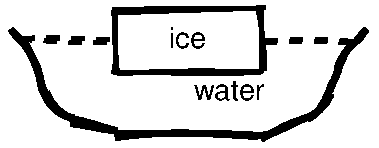
\includegraphics{../docs/fig/bathtub.pdf}
\caption{Ice in a Bathtub}
\label{f:models-bathtub}
\end{figure}

The correct answer is that the level stays the same: the ice displaces
its own weight in water, so it exactly fills the ``hole'' it has made
when it melts. Figuring out why helps people build a model of the
relationship between weight, volume, and density \cite{Epst2002}.

Describe another kind of formative assessment you have seen or used and
explain how it helps both the instructor and the learner figure out
where they are and what they need to do next.

\exercise{A Different Progression}{individual}{15}

The model of skill development described at the start of this chapter
is sometimes called the
\href{https://en.wikipedia.org/wiki/Dreyfus_model\_of\_skill\_acquisition}{Dreyfus
  model}.  Another commonly-used progression is the
\href{https://en.wikipedia.org/wiki/Four_stages_of_competence}{four
  stages of competence}:

\begin{description}

  \item[Unconscious incompetence:] the person doesn't know what they
    don't know.

  \item[Conscious incompetence:] the person realizes that they don't
    know something.

  \item[Conscious competence:] the person has learned how to do
    something, but can only do it while concentrating, and may still
    need to break things down into steps.

  \item[Unconscious competence:] the skill has become second nature,
    and the person can do it reflexively.

\end{description}

\noindent
Identify one subject where you are at each level.  What level are most
of your learners at?  What level are you trying to get them to?

\exercise{What Kind of Book Is This?}{small groups}{5}

What are the chapters in the main body of this book: a tutorial or a
manual?  What about the appendices?  Why?

\exercise{What Kind of Computing?}{individual}{10}

\cite{Tedr2008} summarizes three traditions in computing:

\begin{description}

\item[Mathematical:] Programs are the embodiment of algorithms; they
  are either correct or incorrect, as well as more or less efficient.

\item[Scientific:] Programs are more or less accurate models of
  information processes that can be studied using the scientific
  method.

\item[Engineering:] Programs are built objects like dams and
  airplanes, and are more or less effective and reliable.

\end{description}

\noindent
Which of these best matches your mental model of computing?  If none
of them do, what model do you have?

\input{memory}
\input{architecture}
\chapter{Aprendizaje individual}\label{s:individual}

Los capítulos previos han explorado cómo las/los docentes pueden ayudar a sus estudiantes.
Este capítulo se enfoca en cómo las/los estudiantes pueden ayudarse a sí mismas/os
al cambiar sus estrategias de estudio y descansar lo necesario.

La estrategia más efectiva es hacer un cambio de \gref{g:passive-learning}{aprendizaje pasivo}
a \gref{g:active-learning}{aprendizaje activo}~\cite{Hpl2018},
ya que mejora la tasa de rendimiento y reduce la tasa de fracaso~\cite{Free2014}:

\begin{longtable}{ll}
\textbf{Pasivo}        & \textbf{Activo} \\
Leer sobre un tema        & Hacer ejercicios \\
Mirar un video            & Discutir un tema \\
Asistir a una clase        & Tratar de explicar un tema
\end{longtable}

\noindent
Si hacemos referencia a nuestro modelo simplificado de arquitectura cognitiva (\figref{f:arch-model}),\index{arquitectura cognitiva}
el aprendizaje activo es más efectivo porque retiene la información nueva en la memoria a corto plazo por más tiempo,\index{memoria a corto plazo}
lo cual aumenta la probabilidad que sea codificada con éxito y almacenada en la memoria a largo plazo.\index{memoria a largo plazo}
Al usar la nueva información a medida que llega,
tus estudiantes pueden construir y fortalecer los lazos entre la información nueva y la información que ya poseen,
lo cual a su vez incrementa las chances de que puedan recuperarla más tarde.

La otra clave para poder sacarle más provecho al aprendizaje es la \gref{g:metacognition}{metacognición}
o, en otras palabras, pensar sobre lo que una/uno está pensando.
Así como las/los músicas/os escuchan lo que están tocando,
y las/los buenas/os docentes reflexionan sobre su enseñanza (\chapref{s:performance}),
tus estudiantes aprenderán mejor y más rápido si hacen planes,
fijan metas
y monitorean su progreso.
Para tus estudiantes es difícil dominar estas habilidades en abstracto---no tiene
ningún efecto decirles simplemente que planifiquen---pero
las lecciones pueden diseñarse para motivar buenas prácticas de estudio.
Al hacer referencia a dichas prácticas en la clase,
ayudas a tus estudiantes a darse cuenta de que aprender es una habilidad que pueden mejorar, como cualquier otra~\cite{McGu2015,Miya2018}.

El gran premio es la \gref{g:transfer-of-learning}{transferencia del aprendizaje},
que ocurre cuando algo que hemos aprendido nos ayuda a aprender algo nuevo más rápido.
Las/los investigadores distinguen entre \grefdex{g:near-transfer}{transferencia cercana}{transferencia del aprendizaje!transferencia cercana},
que ocurre entre áreas similares o relacionadas como las fracciones y decimales en matemáticas,
y \grefdex{g:far-transfer}{transferencia lejana}{transferencia del aprendizaje!transferencia lejana},
que ocurre entre dominios diferentes---por ejemplo,
la idea de que aprender ajedrez ayudará al razonamiento matemático y viceversa.

La transferencia cercana ocurre indudablemente---ningún tipo de aprendizaje
más allá de la simple memorización podría ocurrir si no fuera así---y
las/los docentes la utilizan todo el tiempo
al dar a sus estudiantes ejercicios similares al material que acaba de ser presentado en la lección.
Sin embargo,
\cite{Sala2017} analizó varios estudios sobre la transferencia lejana
y concluye que:

\begin{quote}

  {\ldots}los resultados muestran un efecto pequeño a moderado.
  Sin embargo, el tamaño del efecto está inversamente relacionado a la calidad del diseño experimental.{\ldots}
  Concluimos que la transferencia lejana raramente sucede.

\end{quote}

Los casos en que la transferencia lejana sí sucede
parecen ocurrir solamente cuando el tema ya ha sido dominado~\cite{Gick1987}.
En la práctica,
esto significa que aprender a programar no ayudará a jugar ajedrez y viceversa.

\seclbl{Seis estrategias}{s:individual-strategies}

Las/los psicólogas/os estudian el aprendizaje en una amplia variedad de formas,
pero han llegado a conclusiones similares sobre qué funciona realmente~\cite{Mark2018}.
Las/Los \hreffoot{http://www.learningscientists.org/}{\emph{Learning Scientists} (Científicos/as del aprendizaje)}
han catalogado seis de estas estrategias y
las resumieron en \hreffoot{http://www.learningscientists.org/downloadable-materials}{una serie de afiches para descargar}\footnote{Los afiches se encuentran en español, busca el botón \emph{posters in other languages} en la web}.
Si enseñas estas estrategias a tus estudiantes,
y las mencionas por su nombre cuando las utilices en la clase,
estarás ayudando a que aprendan cómo aprender más rápido y mejor~\cite{Wein2018a,Wein2018b}.

\subsection*{Práctica distribuida}
\index{práctica distribuida (estrategia de aprendizaje)}
\index{estrategia de aprendizaje!práctica distribuida}

Diez horas de estudio repartidas en cinco días
es más efectivo que dos días de estudio con cinco horas,
y mucho mejor que un día de diez horas.
Por lo tanto, deberías crear un cronograma de estudio en el que distribuyas tus actividades de estudio a lo largo del tiempo:
reserva al menos media hora para estudiar cada tema, cada día,
en vez de amontonar todo para la noche antes del examen~\cite{Kang2016}.

También deberías revisar los materiales después de cada clase,
pero no inmediatamente después---toma al menos media hora de receso.
Cuando repases,
asegúrate de incluir aunque sea un pequeño porcentaje del material anterior:
por ejemplo,
utiliza veinte minutos para revisar las notas de la clase de hoy
y luego cinco minutos para revisar material de los días anteriores
y de la semana pasada.
Esto te ayudará a identificar algún vacío o errores en tus apuntes previos
cuando todavía haya tiempo para corregirlos o hacer preguntas:
es doloroso darse cuenta la noche del examen
de que no tienes idea por qué subrayaste ``¡¡Evaluación no estándar!!'' tres veces.

Al repasar,
haz notas sobre las cosas que te hayas olvidado:
por ejemplo,
haz una tarjeta de memoria para cada concepto que no pudiste recordar
o que recordaste incorrectamente~\cite{Matt2019}.
Esto te ayudará a enfocarte en aquello que necesite más atención cuando vuelvas a estudiar.

\begin{aside}{El valor de las clases magistrales}
  Según~\cite{Mill2016a},
  ``Las clases magistrales que predominan en los cursos presenciales son formas relativamente ineficientes de enseñar,
  pero probablemente contribuyen a distribuir el material en los momentos correctos,
  porque se desenvuelven en un cronograma pre\-establecido.
  Por el contrario,
  dependiendo de cómo se organicen los cursos,
  las/los estudiantes en línea a veces pueden evitar exponerse al material por completo hasta que una tarea esté cerca.''
\end{aside}

\subsection*{La práctica de recordar lo aprendido}
\index{práctica de recordar lo aprendido (estrategia de aprendizaje)}
\index{estrategia de aprendizaje!práctica de recordar lo aprendido}

El factor limitante de la memoria a largo plazo no es \emph{retener} (qué se almacena)
sino \emph{recordar} (qué puede accederse).
La habilidad de recordar una información específica puede entrenarse,
asi que para mejorar los resultados en situaciones reales
es útil hacer exámenes de práctica o resumir en detalle un tema de memoria
y luego revisar qué has recordado y qué no.
Por ejemplo,
\cite{Karp2008} encontró que hacer exámenes de forma repetida mejora el recuerdo de listas de palabras, de un 35\% a un 80\%.

La habilidad de recordar mejora cuando en la práctica se utilizan actividades similares a las que se evalúan.
Por ejemplo,
escribir entradas en un diario personal ayuda con las preguntas de opción múltiple,
aunque menos que hacer exámenes de práctica~\cite{Mill2016a}.
Este fenómeno se llama
\gref{g:transfer-appropriate-processing}{transferencia apropiada de procesamiento}.

Una manera de ejercitar las habilidades para recordar es resolver un mismo problema dos veces.
La primera vez,
hacerlo completamente de memoria, sin notas o discusiones con pares.
Después de evaluar tu propio trabajo con una rúbrica de respuestas distribuidas por la/el docente,
resuelve el problema de nuevo, utilizando el material de apoyo que quieras.
La diferencia entre ambos te muestra qué tan bien pudiste recordar y aplicar el conocimiento.

Otro método (mencionado previamente) es crear tarjetas de estudio.
Las tarjetas físicas tienen una pregunta en un lado y la respuesta en el otro,
y existen muchas aplicaciones para generarlas disponibles para teléfono móvil.
Si estás estudiando en grupo,
intercambiar las tarjetas de estudio con tus colegas
te ayudará a descubrir ideas importantes que tal vez habías obviado o malinterpretado.

\gref{g:read-cover-retrieve}{Leer-cubrir-recordar}{leer-cubrir-recordar}
es una alternativa rápida a las tarjetas de estudio.
Mientras lees algo,
cubre los términos clave o secciones con notas adhesivas pequeñas.
Cuando hayas terminado,
vuelve a leer y ve qué tan bien puedes adivinar las palabras cubiertas por las notas adhesivas.
Independientemente del método que uses,
no sólo practiques recordar datos y definiciones:
asegúrate de evaluar la comprensión de grandes ideas 
y de las conexiones entre ellas.
Una forma rápida de hacer esto es
diseñar un mapa conceptual y compararlo con tus apuntes
o con un mapa conceptual dibujado previamente.

\begin{aside}{Hipercorrección}
    Un descubrimiento poderoso en la investigación del aprendizaje es
  el \gref{g:hypercorrection}{fenómeno de hipercorrección}~\cite{Metc2016}.
  A la mayoría de las personas no le gusta que le digan cuando dicen algo incorrecto,
  así que sería razonable asumir que
  mientras más confianza tenga una persona en la respuesta que da en un examen,
  más difícil será cambiar su opinión si el resultado era incorrecto.
  Y resulta que lo opuesto es cierto:
  mientras más confianza tenga una persona en que tiene la razón,
  más probable será que no repita el error si recibe una corrección.
\end{aside}

\subsection*{Práctica intercalada}
\index{práctica intercalada (estrategia de aprendizaje)}
\index{estrategia de aprendizaje!práctica intercalada}

Una forma de espaciar la práctica es intercalar el estudio de diferentes temas:
en vez de dominar un tema,
luego el segundo y el tercero,
alterna las sesiones de estudio.
Aún mejor,
cambia el orden:
A-B-C-B-A-C es mejor que A-B-C-A-B-C,
que a la vez es mejor que A-A-B-B-C-C~\cite{Rohr2015}.
Esto funciona porque intercalar permite la creación de más vínculos entre los diferentes temas,
lo cual mejora el aprendizaje.

Cuánto deberías tardar en cada ítem
depende del tema y de qué tan bien lo conozcas.
Entre 10 y 30 minutos es un tiempo suficiente para
entrar en tema (\secref{s:individual-time})
pero no para deambular.
Al principio, intercalar el estudio parecerá más difícil que enfocarse en un único tema,
pero ese es un signo de que está funcionando.
Si usas tarjetas de estudio o haces exámenes de práctica para medir tu progreso,
deberías ver una mejora después de un par de días.

\subsection*{Elaboración}
\index{elaboración (estrategia de aprendizaje)}
\index{estrategia de aprendizaje!elaboración}

Explicarte los temas a tí misma/o mientras estudias
permite entenderlos y recordarlos.
Una forma de hacer esto es complementar la respuesta en un examen práctico
con la explicación de por qué la respuesta es correcta
o, al contrario, con una explicación de por qué otras respuestas plausibles no serían correctas.
Otra alternativa es decirte a tí misma/o
cómo una nueva idea es similar o diferente a una que ya hayas visto previamente.

Si bien hablarte a tí misma/o puede parecer una forma extraña de estudiar,
~\cite{Biel1995} encontró que
las personas entrenadas en auto-explicarse destacan cuando se comparan con quienes no se entrenaron.
De manera similar,
\cite{Chi1989} encontró que algunas/os estudiantes simplemente frenan cuando se encuentran con un paso que no entienden
al tratar de resolver problemas.
Otras personas paran y generan una explicación de lo que está pasando:
así aprenden más rápido.
Un ejercicio para construir esta habilidad es revisar un ejemplo de programación línea por línea con una clase, de modo 
que diferentes personas expliquen cada línea
y digan por qué está ahí y qué es lo que produce.

\subsection*{Ejemplos concretos}
\index{ejemplos concretos (estrategia de aprendizaje)}
\index{estrategia de aprendizaje!ejemplos concretos}

Una forma particularmente útil de la estrategia de aprendizaje de elaboración es el uso de ejemplos concretos.
Cuando se tiene una definición de un principio general,
intenta proveer uno o más ejemplos de su uso
o, por el contrario, toma un problema en particular y enuncia los principios generales que representa.
\cite{Raws2014} encontró que intercalar ejemplos y definiciones de esta forma
permite que las/los estudiantes puedan recordar las definiciones correctamente.

Una forma estructurada de hacer esto es con
el \hreffoot{https://betterexplained.com/articles/adept-method/}{método ADEPT}:
\index{ADEPT (patrón de lección)}
\index{patrón de lección!ADEPT}
da una \textbf{A}nalogía,
dibuja un \textbf{D}iagrama,
presenta un \textbf{E}jemplo,
describe la idea en un lenguaje \textbf{S}encillo (del inglés \emph{"\textbf{P}lain Language"}),
y luego da los detalles \textbf{T}écnicos.
De nuevo,
si estás estudiando con otra persona o en grupo,
puedes intercambiar y revisar el trabajo:
ve si estás de acuerdo con el ejemplo que tus pares eligieron para representar
el principio que se está discutiendo,
o analiza qué principios se usan en un ejemplo que no hayan anotado.

Otra técnica útil es enseñar por contraste,
\index{enseñar por contraste (patrón de lección)}
\index{patrón de lección!enseñar por contraste}
p.ej.\ mostrar a tus estudiantes cuál \emph{no} es la solución
o cuál es la técnica que \emph{no} resolverá un problema.
Por ejemplo,
al mostrar a las/los niñas/os cómo simplificar fracciones,
es importante darles a menos un par de ejemplos que no puedan simplificarse, como 5/7,
para que no se frustren buscando respuestas que no existen.

\subsection*{Programación dual}
\index{programación dual (estrategia de aprendizaje)}
\index{extrategia de aprendizaje!programación dual}

La última de las seis estrategias principales
descriptas en \hreffoot{http://www.learningscientists.org/}{\emph{Learning Scientists}}
es presentar palabras e imágenes juntas.
Como discutimos en la \secref{s:architecture-brain},
diferentes subsistemas en nuestro cerebro manejan y almacenan la información lingüística y visual,
de tal manera que, si se presenta información complementaria por ambos canales,
se refuerzan mutuamente.
Sin embargo,
aprender es menos efectivo cuando la misma información se presenta de forma simultánea por dos canales diferentes,
porque el cerebro tiene que hacer un esfuerzo para comparar los canales entre sí~\cite{Maye2003}.

Una forma de aprovechar la programación dual es dibujar o etiquetar líneas de tiempo,
mapas o árboles familiares,
o cualquier otro material que sea relevante.
(Personalmente, me gustan las imágenes que muestran qué funciones llaman a qué otras en un programa.)
Dibujar un diagrama \emph{sin} etiquetas,
y después volver atrás para etiquetarlo,
es una práctica excelente para recordar.

\seclbl{Gestión del tiempo}{s:individual-time}

Solía presumir sobre la cantidad de horas que trabajaba.
No en muchas palabras,
obviamente---tenía \emph{algunas} habilidades sociales---pero
me presentaba en clases alrededor del mediodía,
sin rasurar y bostezando,
y casualmente mencionaba a quien sea que pudiera escuchar
que había trabajado toda la noche.

Haciendo memoria,
no puedo recordar a quién trataba de impresionar.
Pero lo que sí recuerdo es
que tuve que desechar gran parte del trabajo que hice durante esas trasnochadas
una vez que lo revisé después de dormir un poco,
Para peor, el trabajo que no descarté le hizo bastante daño a mis calificaciones.

Mi error fue confundir ``trabajar'' con ``ser productivo.''
No puedes producir software (o cualquier otra cosa) sin hacer algo de trabajo,
pero se puede hacer mucho trabajo sin producir nada de valor.
Convencer de esto a otras personas es difícil,
especialmente cuando son adolescentes o tienen alrededor de veinte años,
pero paga tremendos dividendos.

Los estudios científicos sobre el trabajo en exceso y la deprivación del sueño se remontan, al menos, a la década de 1890s---puedes ver
\cite{Robi2005} para un resumen breve y legible.\index{trabajo en exceso}\index{privación del sueño}
Los resultados más importantes para estudiantes son:

\begin{enumerate}

\item
  Trabajar más de 8 horas al día por un periodo extendido de tiempo
  disminuye la productividad total,
  no sólo la productividad por hora ---es decir, haces menos en total (no sólo por hora)
  cuando tienes trabajo acumulado y estás cerca de una fecha límite de entrega.

\item
  Trabajar durante 21 horas seguidas aumenta la posibilidad de que tengas un error catastrófico
  tanto como estar legalmente en estado de ebriedad.

\item
  La productividad varía a lo largo de la jornada laboral,
  con la mayor productividad en las primeras 4 a 6 horas.
  Después de cierta cantidad de horas,
  la productividad disminuye a cero;
  y eventualmente se vuelve negativa.

\end{enumerate}

Estos hechos se han reproducido y verificado durante más de un siglo,
y los datos detrás de ellos son tan sólidos como los que relacionan el tabaquismo con el cáncer de pulmón.
El problema es que
\emph{las personas generalmente no notan que sus habilidades disminuyen}.
Al igual que las personas que en estado de ebriedad creen que todavía pueden conducir,
las personas que están deprivadas de sueño no se dan cuenta de que
no están terminando sus oraciones (o pensamientos).
Se ha demostrado que cinco días de 8 horas por semana maximizan la producción total a largo plazo
en todas las industrias que se han analizado;
estudiar o programar no es diferente.

Pero, ¿qué pasa con las rachas que surgen de vez en cuando,
como trabajar toda la noche para cumplir con un plazo?
Eso también se ha estudiado
y los resultados no son agradables.
La habilidad de pensar disminuye en un 25\% por cada 24 horas sin dormir.
Puesto de otra forma,
el coeficiente intelectual de una persona promedio es sólo 75 después de una trasnochada,
lo que la desplaza al 5\% inferior de la población.
Si haces dos trasnochadas seguidas, tu coeficiente intelectual es de 50,
que es el nivel en el que las personas suelen ser consideradas incapaces de vivir de forma independiente.

``Pero---pero---, ¡tengo tantas tareas que hacer!'' dices.
``¡Y todas tienen que ser entregadas al mismo tiempo!
¡\emph{Tengo} que trabajar horas extra para completarlas!''
No:
para ser productivas las personas tienen que priorizar tareas y enfocarse,
lo cual se les debe enseñar.
Una técnica ampliamente utilizada es hacer una lista de tareas a hacer,
organizadas por prioridad,
y luego desconectarse del correo electrónico u otras interrupciones por 30--60 minutos
y completar una de esas tareas.
Si una de las tareas de la lista lleva más de una hora,
sepárala en actividades más pequeñas y priorízalas de forma separada.

La parte más importante de esto es apagar las interrupciones.
A pesar de lo que mucha gente quiere creer,
los seres humanos no somos buenos haciendo múltiples tareas a la vez.\index{múltiples tareas}.
En lo que sí podemos volvernos buenos es en la \gref{g:automaticity}{automaticidad}, es decir, 
la habilidad de hacer algo de forma rutinaria de fondo,
mientras realizamos otra tarea~\cite{Mill2016a}.
La mayoría de las personas puede hablar mientras corta una cebolla,
o tomar café mientras lee;
con la práctica,
también podemos tomar notas mientras escuchamos,
pero no podemos estudiar de forma efectiva,
programar
o hacer otra tarea mentalmente exigente mientras prestamos atención a algo más---solo
creemos que podemos.

El objetivo de organizarse y prepararse es
entrar en el estado mental más productivo posible.
Las/los psicólogas/os lo llaman \gref{g:flow}{flujo}~\cite{Csik2008};
las/los atletas lo llaman ``estar en la zona,''
y las/los músicos hablan de perderse en lo que están tocando.
Cualquiera sea el nombre que uses,
las personas producen mucho más por unidad de tiempo en este estado que en un estado normal.
La mala noticia es que
se tarda aproximadamente 10 minutos en volver a entrar en este estado después de tener una interrupción,
sin importar lo corta que haya sido la interrupción.
Lo que significa que si te interrumpieron seis veces por hora,
\emph{nunca} llegaste al máximo de tu productividad.


\begin{aside}{¿Cómo lo supo?}

  En su breve historia en 1961 ``\hreffoot{https://en.wikipedia.org/wiki/Harrison\_Bergeron}{Harrison Bergeron}, ''Kurt Vonnegut describió un futuro en el que las personas están obligadas a ser iguales.
  Las personas atractivas tienen que usar máscaras,
  las personas atléticas tienen que cargar pesas---y las personas inteligentes
  están obligadas a llevar radios que interrumpen sus pensamientos en intervalos aleatorios.
  A veces me pregunto si---oh, un momento, mi teléfono acaba de---perdón, ¿de qué estábamos hablando?

\end{aside}

\seclbl{Evaluación de pares}{s:individual-peer}
\index{evaluación de pares}

Pedirle a las personas de un equipo que evalúen a sus pares es una práctica común en la industria.
\cite{Sond2012} revisaron la literatura sobre evaluación de pares,
distinguiendo entre calificar y evaluar.
Descubrieron que la evaluación de pares aumentaba la cantidad, la diversidad y la puntualidad de la retroalimentación,
ayudaba a las/los estudiantes a ejercitar el pensamiento de nivel superior,
fomentaba la práctica reflexiva,
y promovía el desarrollo de habilidades sociales.
Las preocupaciones fueron predecibles:
validez y confiabilidad,
motivación y procrastinación,
agresión, confabulación y plagio.

Sin embargo,
la evidencia muestra que estas preocupaciones no fueron significativas en la mayoría de las clases.
Por ejemplo,
\cite{Kauf2000} comparó las evaluaciones y calificaciones confidenciales de pares en varios ejes
para dos cursos en licenciatura en ingeniería,
y descubrió que la auto-calificación y la evaluación de pares tuvo una concordancia estadística,
que la confabulación no fue significativa (es decir, no dieron irrespectivamente la nota más alta a todos sus pares),
que las/los estudiantes no inflaron sus auto-calificaciones
y, lo más importante,
que las calificaciones no estaban sesgadas por cuestiones de género ni por racismo.

Una forma de implementar la evaluación de pares es \gref{g:contributing-student-pedagogy}{contribuyendo a la pedagogía estudiantil},
en la cual tus estudiantes producen artefactos para contribuir al aprendizaje de otros.
Esto puede hacerse desarrollando una lección corta y compartiéndola con la clase,
contribuir a un banco de preguntas,
o escribir notas de una lección en particular para una publicación durante la clase.
Por ejemplo,
\cite{Fran2018} evidenció que las/los estudiantes que realizan videos cortos para enseñar conceptos a sus pares
tuvieron un incremento significativo de su propio aprendizaje
comparado al de aquellas personas que sólo estudiaron el material o vieron los videos.
He observado que pedir a diario a mis estudiantes que compartan a la clase un error en su código 
y cómo lo solucionaron ayuda en sus habilidades analíticas y disminuye su síndrome del impostor/a.

Otra alternativa es la \gref{g:calibrated-peer-review}{revisión por pares calibrada},
en la cual tus estudiantes revisan uno o más ejemplos utilizando una rúbrica
y comparan su evaluación con la evaluación del cuerpo docente~\cite{Kulk2013}.
Una vez que la evaluación de tu estudiante sea similar a la del cuerpo docente,
pueden empezar a evaluar el trabajo de sus pares.
Si se combinan muchas evaluaciones de pares,
este método puede ser tan preciso como la evaluación del cuerpo docente ~\cite{Pare2008}.

Como todo lo demás,
la evaluación es ayudada por rúbricas.
La planilla de evaluación de la \secref{s:checklists-teameval} muestra un ejemplo para que puedas empezar.
Para usarla,
evalúate y luego evalúa a tus colegas,
luego calcula y compara las notas.
Una diferencia grande generalmente indica la necesidad de más conversación.

\seclbl{Ejercicios}{s:individual-exercises}

\exercise{Estrategias de aprendizaje}{individual}{20’}

\begin{enumerate}

\item
  ¿Cuál de las seis estrategias de aprendizaje generalmente usas?
  ¿Cuáles generalmente no usas?

\item
  Escribe tres conceptos generales que quieras que tus estudiantes aprendan
  y da dos ejemplos específicos para cada caso
  (practica ejemplos concretos).
  Para cada uno de estos conceptos,
  trabaja al revés: parte de uno de los ejemplos y elabora sobre el concepto que lo explica
  (elaboración).

\end{enumerate}

\exercise{Conectando ideas}{parejas}{5’}

Este ejercicio es un ejemplo de utilizar la elaboración para mejorar la retención.
Tú y tu pareja deben elegir una idea de manera independiente.
Luego de contarse sus ideas,
trata de encontrar una cadena de cuatro eslabones
que las conecte.

Por ejemplo,
si las dos ideas son ``Titicaca'' y ``estadística,''
los eslabones pueden ser:

\begin{itemize}

\item
  El lago Titicaca se encuentra en territorios de Bolivia y Perú;

\item
  Bolivia y Perú son países;

\item
 los países tienen gobiernos;

\item
  los gobiernos utilizan estadísticas para analizar la opinión pública.

\end{itemize}

\exercise{Evolución convergente}{parejas}{15’}

Una práctica que no hemos abordado anteriormente son las \gref{g:guided-notes}{notas guiadas}.
Se trata de notas preparadas por la/el docente,
quien solicita a sus estudiantes que respondan preguntas respecto a la información clave de una clase magistral o discusión.
Estas preguntas pueden ser espacios en blancos donde tus estudiantes agregan información,
asteriscos junto a términos que deben definir,
etcétera.

Crea entre dos y cuatro tarjetas con notas guiadas para una lección que hayas enseñado recientemente
o que vas a enseñar.
Intercambia tarjetas con tu colega:
¿Qué tan fácil es entender lo que se está preguntando?
¿Cuánto tiempo te lleva completar las respuestas?
¿Qué tan bien funciona esto para ejemplos de programación?

\exercise{Cambiando de opinión}{parejas}{10’}

\cite{Kirs2013} argumentan que los mitos sobre personas nativas digitales,
estilos de aprendizaje,
y personas autodidactas se derivan de una misma creencia equivocada: que
las/los estudiantes saben lo que es mejor para ellas/os.
Los autores advierten que podemos estar en una espiral descendente
en la que todos los intentos de los/las investigadoras/es en educación para refutar estos mitos
confirmen la creencia de sus oponentes de que la ciencia de aprendizaje es pseudociencia.
Elige algo que hayas aprendido hasta ahora en este libro,
que te haya sorprendido o haya contradecido algo que creías previamente,
y practica explicar esa idea a tu colega en 1--2 minutos.
¿Cuán convincente eres?

\exercise{Tarjetas de estudio}{individual}{15’}

Utiliza notas adhesivas, o algo similar que tengas a mano,
para hacer seis tarjetas de estudio
para un tema que recientemente hayas enseñado o aprendido.
Intercambia con tu colega y ve cuánto tiempo tardas en recordar
al 100\% cada tarjeta.
Deja las tarjetas a un lado cuando termines
y vuelve media hora después para evaluar cuál es tu tasa de retención.

\exercise{Utilizando ADEPT}{toda la clase}{15’}

Elige un tema que recién hayas enseñado o aprendido,
y delinea una pequeña lección que utilice los cinco pasos del método ADEPT para introducir el tema.

\exercise{El costo de la multitarea}{parejas}{10’}

\hreffoot{http://www.learningscientists.org/blog/2017/7/28-1}{El blog de \emph{The Learning Scientists}}
describe un experimento simple que puedes hacer con solo un cronómetro
para demostrar el costo de hacer múltiples tareas a la vez.
En parejas,
mide cuánto tarda cada persona en hacer cada una de estas tres tareas:

\begin{itemize}
\item
  Contar del 1 al 26 dos veces.
\item
  Recitar el alfabeto de la A a la Z dos veces.
\item
  Intercalar números y letras,
  es decir, ``1, A, 2, B, {\ldots}''
  y continuar.
\end{itemize}

Luego, cada pareja informa sus tiempos a la clase.
Sin práctica específica,
intercalar números y letras siempre toma significativamente más tiempo que cada uno de los componentes por separado.

\exercise{Mitos en la educación de computación}{toda la clase}{20'}

\cite{Guzd2015b} presenta una lista de las 10 creencias erróneas más comunes sobre educación en computación,
que incluye:

\begin{enumerate}
\item
  La ausencia de mujeres en ciencias de la computación es similar a lo que ocurre en otras áreas de ciencias, tecnología, ingeniería y matemáticas.
\item
  Para tener más mujeres en las ciencias de la computación necesitamos más docentes mujeres en el área.
\item
  Las evaluaciones de estudiantes son la mejor forma de evaluar la enseñanza.
\item
  Las/los buenas/os docentes personalizan la educación a los estilos de aprendizaje de sus estudiantes.
\item
  Las/los buenas/os docentes en ciencias de la computación deberían modelar buenas prácticas 
  de desarrollo de software porque su trabajo es producir ingenieras/os de software excelentes.
\item
  Algunas personas son naturalmente mejores programadoras que otras.
\end{enumerate}

Cada persona de la clase es invitada a votar +1 (de acuerdo), -1 (en desacuerdo) o 0 (neutro) para cada punto.
Luego, la/el docente lee la explicación completa en
\hreffoot{https://cacm.acm.org/blogs/blog-cacm/189498-top-10-myths-about-teaching-computer-science/fulltext}{el artículo original}
y se vuelve a hacer la votación.
¿En cuáles preguntas las personas cambiaron de parecer?
¿Cuáles todavía creen que son verdad, y por qué?

\exercise{Revisión por pares calibrada}{parejas}{20’}

\begin{enumerate}

\item
  Crea una rúbrica de 5--10 puntos
  con entradas como ``buenos nombres de variables,'' ``sin código redundante,'' y ``flujo de control propiamente anidado''
  para calificar el tipo de programa que esperarías que tus estudiantes escriban.

\item
  Elige o crea un pequeño programa que contenga 3--4 violaciones a estas entradas.

\item
  Califica el programa de acuerdo a la rúbrica.

\item
  Pide a tu colega que califique el mismo programa con la misma rúbrica.
  ¿Qué aceptó tu colega pero tú no aceptaste?
  ¿Qué criticó tu colega pero tú no criticaste?

\end{enumerate}

\section*{Revisión}

\figpdfhere{figures/conceptmap-active-learning.pdf}{Conceptos: Aprendizaje activo}{f:individual-concept-map}

\input{process}
\input{pck}
\input{performance}
\input{classroom}
\chapter{Motivación y desmotivación}\label{s:motivation}

Los/las estudiantes necesitan ánimo para enfrentar terreno desconocido,
así que este capítulo analiza maneras en las que el cuerpo docente puede motivarlos/las.
Y más importante,
el capítulo habla de cómo los/las docentes pueden desmotivarlos/as
y cómo evitarlo.

Nuestro punto de partida es la diferencia entre
\gref{g:extrinsic-motivation}{motivación extrínseca},
lo que sentimos cuando hacemos algo para evitar un castigo o ganarnos una recompensa,
y \gref{g:intrinsic-motivation}{motivación intrínseca},
lo que sentimos cuando conseguimos algo que nos satisface personalmente.
Ambos tipos de motivación nos afectan en la mayoría de las situaciones---por ejemplo,
las personas enseñan porque les gusta y porque les pagan---; pero
aprendemos mejor cuando estamos motivados/as intrínsecamente~cite{Wlod2017}.
De acuerdo a la 
\hreffoot{https://es.wikipedia.org/wiki/Teor'ía\_de\_la\_autodeterminaci'ón}{teoría de la autodeterminación},
los tres impulsores de motivación intrínseca son:

\begin{description}

\item[Competencia:]
  la sensación de que sabes lo que haces. \index{motivación!competencia}

\item[Autonomía:]
  la sensación de estar en control de tu propio destino.\index{motivación!autonomía}

\item[Relación:]
  la sensación de estar conectado/a con las demás personas.\index{motivación!relación}

\end{description}

Una lección bien diseñada fomenta estos tres impulsores.
Por ejemplo,
un ejercicio de programación puede permitir que los/las estudiantes
practiquen con las herramientas que necesitan usar para resolver un problema mayor (competencia),
aborden las partes del problema en el orden que quieran (autonomía),
y conversen con sus pares (relación).

\begin{aside}{El problema de las notas}
  Yo nunca he tenido un público en mi vida. Mi público es una rúbrica.\\
  -- citado por \hreffoot{https://twitter.com/figuralities/status/987330064571387906}{Matt Tierney}

 Las calificaciones y la forma en que distorsionan el aprendizaje se utilizan con frecuencia como ejemplo de motivación extrínseca,
  pero como observa~\cite{Mill2016a},
  no van a desaparecer en el corto plazo,
  así que no tiene sentido intentar construir un sistema que las ignore.
  En lugar de eso,~\cite{Lang2013} explora cómo los cursos que enfatizan las calificaciones
  pueden incentivar a que los/las estudiantes hagan trampa
  y ofrece algunos consejos de cómo disminuir este efecto,
  mientras~\cite{Covi2017} observa el problema más grande de
  balancear la motivación intrínseca y extrínseca en la educación institucional,
  y el enfoque de \hreffoot{https://en.wikipedia.org/wiki/Constructive\_alignment}{alineación constructiva}
  defendido en~\cite{Bigg2011} busca armonizar las actividades de aprendizaje con los resultados del aprendizaje.
\end{aside}

\cite{Ambr2010} contiene una lista de métodos basados en evidencia para motivar a los/las estudiantes.
Ninguno es sorprendente, es
difícil imaginar a alguien diciendo que \emph{no debemos} identificar y recompensar lo que valoramos, pero
es útil revisar lecciones para asegurarnos de que estén haciendo al menos algunas de estas cosas.
Una estrategia en particular que me gusta es
que los/las estudiantes que hayan luchado y tenido éxito
se acerquen y cuenten sus historias al resto de la clase.
Es más probable que tus estudiantes crean historias de personas parecidas a ellos/as~\cite{Mill2016a}
y, además, quienes ya han pasado por tu curso
siempre tendrán consejos en los que nunca hubieras pensado.

\begin{aside}{No solo para estudiantes}
  Las discusiones sobre motivación en educación con frecuencia pasan por alto la necesidad de motivar al \emph{docente}.\index{motivación!de docentes}
  Los/las estudiantes responden al entusiasmo de su docente,
  y los/las docentes (particularmente si el trabajo es voluntario) necesitan valorar un tema para seguir enseñándolo. 
  Esta es otra razón poderosa para co-enseñar (\secref{s:classroom-together}):
  al igual que tener un/una compañero/a para correr hace que sea más probable que sigas corriendo,
  tener un/una compañero/a docente ayuda a ponerte en marcha
  esos días que tienes una gripe
  y la bombilla del proyector se ha roto
  y nadie sabe donde conseguir un reemplazo
  y, ¿de verdad están construyendo \emph{otra vez}?
\end{aside}

Los/las docentes también pueden hacer otras cosas positivas.
\cite{Bark2014} registró tres cosas que impulsaron la retención para todos los/las estudiantes:
tareas significativas,
interacción del cuerpo docente con los/las estudiantes
y colaboración entre estudiantes en las tareas.
El ritmo y la carga de trabajo relativo a las expectativas también fueron impulsores significativos,
pero principalmente para estudiantes varones.
Las cuestiones que \emph{no} impulsaron la retención
fueron: interactuar con asistentes de la clase
e interactuar con compañeros/as en actividades extracurriculares.
Estos resultados parecen obvios,
pero lo contrario también parecería obvio:
si el estudio hubiera concluido que compartir actividades extracurriculares
impulsa la retención,
también pensaríamos que tiene sentido.
Notablemente,
replicar en línea a dos de los cuatro impulsores de retención (interacción  con el cuerpo docente y colaboración entre estudiantes)
toma un esfuerzo adicional (\chapref{s:online}).

\seclbl{Tareas auténticas}{s:motivation-authentic}

Como Dylan Wiliam menciona en~\cite{Hend2017},\index{Wiliam, Dylan}
la motivación no siempre conduce al logro 
pero el logro casi siempre conduce a la motivación:
el éxito de los/las estudiantes les motiva mucho más a que les digan lo maravillosos/as que son.
Podemos usar esta idea en la docencia
creando una cuadrícula cuyos ejes son ``tiempo medio para dominar''
y ``utilidad una vez dominado'' (\figref{f:motivation-what}).

\figpdf{figures/what-to-teach.pdf}{Qué enseñar}{f:motivation-what}

Las cosas que se dominan rápido y son útiles de inmediato se deben enseñar primero,
incluso si no se consideran fundamentales para personas que ya son practicantes competentes,
porque unas pocas victorias iniciales fortalecerán la confianza de tus estudiantes en sí mismos/as y en su docente.
Por el contrario.
aquellas cosas que son difíciles de aprender y no son útiles a tus estudiantes en su etapa actual de desarrollo
deben omitirse por completo,
mientras que los temas en la diagonal se deben sopesar entre sí.

\newpage
\begin{aside}{¿Útil para quién?}
  Si alguien quiere construir sitios web,
  conceptos de ciencia de computación fundamentales como recursión y computabilidad
  pueden habitar la esquina inferior derecha de esta cuadrícula. 
  Eso no quiere decir que no vale la pena aprenderlos,
  pero si nuestro objetivo es motivar a las personas,
  pueden y deben ser enseñados diferidos.
  Por lo contrario,
  un/a estudiante de último año tomando un clase de programación para estimular su mente
  puede preferir explorar estas grandes ideas en vez de hacer algo práctico.
  Cuando estás creando tu cuadrícula,
  deberías hacerlo con tus personas tipo en mente
  (Section~\ref{s:process-personas})
  Si los temas se ordenan en lugares muy diferentes para diferentes personas tipo,
  deberías pensar en crear cursos diferentes.
\end{aside}

Un ejemplo bien estudiado de priorizar lo que es útil
sin sacrificar lo que es fundamental
es el enfoque de computación de medios desarrollado en Georgia Tech~\cite{Guzd2013}.\index{computación de medios}
En vez de imprimir ``hola mundo'' o sumar los primeros diez enteros,
el primer programa de un/a estudiante podría ser abrir una imagen,
cambiarle el tamaño para crear una versión miniatura
y guardar el resultado.
Esta es una \gref{g:authentic-task}{tarea auténtica}; 
es decir, algo que los/las estudiantes creen que harían en la vida real.
También tiene un \gref{g:tangible-artifact}{artefacto tangible}:
si la imagen sale del tamaño incorrecto,
los/las estudiantes tienen algo a mano que puede guiar su depuración.
\cite{Lee2013} describe una adaptación de este enfoque de \emph{Python} a MATLAB,
mientras que otras personas están construyendo cursos similares acerca de ciencia de datos, procesamiento de imágenes
y biología~\cite{Dahl2018,Meys2018,Ritz2018}

Siempre habrá tensión entre darle a tus estudiantes problemas auténticos
y ejercitar las habilidades individuales que requieren para resolver esos problemas:
al fin y al cabo,
los/las programadores no contestan preguntas de opción múltiple en el trabajo
como tampoco los/las músicos/as tocan escalas una y otra vez en frente de un público.
Conseguir el balance es difícil,
pero un primer paso es eliminar cualquier cosa arbitraria o sin sentido.
Por ejemplo,
los ejemplos de programación no deben utilizar variables llamadas \texttt{foo} y \texttt{bar},
y si vas a hacer que tus estudiantes ordenen una lista,
haz una lista de canciones en vez de cadenas de caracteres como ``aaa'' y ``bbb''.

\seclbl{Desmotivación}{s:motivation-demotivation}

\begin{quote}

  Las mujeres no abandonan la computación porque no saben cómo es;
  se van porque \emph{sí saben}. \\
  --- atribuido a varias personas

\end{quote}

Si enseñas en un ambiente free-range
probablemente tus estudiantes son voluntarios/as
y probablemente quieren estar en tu clase.
Por lo tanto, motivarlos/as es menos preocupante que desmotivarlos/as.
Desafortunadamente,
es fácil desmotivar a las personas accidentalmente.
Por ejemplo,
\cite{Cher2009} reportaron cuatro estudios mostrando que\index{desmotivación!causas ambientales}
hay pistas ambientales sutiles con una diferencia medible en el interés que las personas de diferentes géneros tienen en la computación:
cambiar los objetos en un aula de ciencias de la computación de aquellos considerados estereotipados de ciencias de la computación
(p.ej.\ afiches y videojuegos de Star Trek)
a objetos no considerados estereotipados (p.ej.\ afiches de la naturaleza y guías telefónicas)
impulsó el interés de estudiantes universitarias al nivel de sus pares masculinos.
De manera similar,
\cite{Gauc2011} reporta tres de estudios que muestran que
la redacción de género comúnmente empleada en materiales de contratación laboral 
puede mantener desigualdad de género en ocupaciones tradicionalmente dominadas por hombres.

Hay tres desmotivadores principales para estudiantes adultos/as:

\begin{description}

\item[Imprevisibilidad:]
  desmotiva a las personas porque
  si no hay una conexión confiable entre lo que hacen y el resultado que logran,
  no hay razón para que intenten hacer nada.\index{desmotivación!imprevisibilidad}


\item[Indiferencia:]
  desmotiva porque
  los/las estudiantes que creen que el/la docente o el sistema educativo no se preocupan por ellos/as,
  no se van a preocupar por aprender la clase.\index{desmotivación!indiferencia}

\item[Injusticia:]
  desmotiva a las personas desfavorecidas por razones obvias.
  Lo sorprendente es que también desmotiva a las personas que se benefician de la injusticia:
  consciente o inconscientemente,
  les preocupa que
  algun dia se encuentren en el grupo desfavorecido~\cite{Wilk2011}.\index{desmotivación!injusticia}

\end{description}

En situaciones extremas,
los/las estudiantes pueden desarrollar \gref{g:learned-helplessness}{indefensión aprendida}:
si están repetidamente sometidos/as a comentarios negativos en una situación que no pueden cambiar,
pueden aprender a ni siquiera intentar cambiar aquello que sí podrían.

Una de las maneras más rápidas y seguras de desmotivar estudiantes es
usar un lenguaje que sugiera que algunas personas son programadoras naturales y otras no.
Guzdial lo ha llamado
\hreffoot{https://cacm.acm.org/blogs/blog-cacm/189498-top-10-myths-about-teaching-computer-science/fulltext}{el mito más grande de enseñar ciencias de la computación},
y \cite{Pati2016} respaldó esto mostrando que
la gente ve evidencia de un ``gen \emph{geek}'' donde no existe uno.\index{gen \emph{geek} (inexistencia de)}
Analizaron distribuciones de calificaciones de 778 cursos universitarios y encontraron que solo 5,8\% mostraba signos
de ser multimodal,
es decir, solo una clase de veinte mostró signos de tener dos poblaciones distintas de estudiantes.
Luego le mostraron a 53 profesores/as de ciencias de la computación histogramas de distribuciones ambiguas de calificaciones;
aquellos/as que creían que algunas personas tienen una predisposición innata a ser mejores en las ciencias de la computación
eran más propensos/as de verlas como bimodal que aquellos/as que no.

Estas creencias son importantes porque los/las docentes actúan sobre ellas~\cite{Brop1983}.
Si un/a docente cree que es probable que a un/a estudiante le vaya bien
naturalmente (a menudo inconscientemente) se enfoca en ese/a estudiante,
que luego cumple con las expectativas debido a la mayor atención,
lo que a su vez parece confirmar la creencia del docente.
Lamentablemente,
hay pocas señales de que la mera evidencia del tipo presentado en \cite{Pati2016}
es suficiente para romper este círculo vicioso{\ldots}

Aquí hay algunas otras cosas específicas que desmotivarán a tus estudiantes:

\begin{description}

\item[Una actitud de superioridad moral o desdeñosa]
  de un/una docente o un/una compañero/a estudiante.

\item[Decirles que sus habilidades existentes son tonterías.]
  Las personas que son usuarias de Unix se burlan de las que usan Windows,
  los/las programadores/as de todo tipo hacen chistes sobre Excel
  y sin importar qué entorno de desarrollo de aplicación web conoces,
  algún/a programador/a te dirá que está desactualizado.
  Seguramente, tus estudiantes invirtieron mucho tiempo y esfuerzo para adquirir las habilidades que tienen;
  menospreciarlas es una buena manera de garantizar que
  no escucharán nada más de lo que tengas que decir.

\item[Sumergirse en discusiones técnicas complejas o detalladas]
  con los estudiantes más avanzados de la clase.

\item[Fingir que sabes más de lo que sabes.]
  Los/las estudiantes confiarán más en ti si hablas con franqueza de los límites de tu conocimiento
  y será más probable que hagan preguntas y pidan ayuda.

\item[Usar la letra S (``solo'') o fingiendo sorpresa.]
  Como se discutió en el \chapref{s:memory},
  decir cosas como ``no puedo creer que no sabes X'' o ``¿nunca has oído de Y?''
  le señala a tus estudiantes que
  piensas que su problema es trivial
  y que deben ser estúpidos/as por no poder resolverlo.

\item[Dolores de cabeza de instalación de software.]
  El primer contacto de las personas con programación o con herramientas nuevas de programación suele a ser desmoralizador
  y creer que algo es difícil de aprender es una profecía autocumplida.
  No es solamente el tiempo que toma en configurar
  o el sentimiento de que es injusto tener que depurar algo que depende de
  precisamente del conocimiento que aún no tienen.
    El problema real es que con cada falla refuerzan su creencia de que
  tendrán una mejor chance de cumplir con la fecha límite del próximo jueves
  si siguen haciendo las cosas como siempre las han hecho.

\end{description}

Es incluso más fácil desmotivar a las personas en línea que en persona,
pero ahora hay estrategias basadas en evidencia para lidiar con esto.
\cite{Ford2016} encontraron que cinco barreras para contribuir en \hreffoot{https://stackoverflow.com/}{Stack Overflow}
sos consideradas significativamente más problemáticas por las mujeres que por los hombres:
falta de conocimiento de las características del sitio,
sentirse incapaz de contestar preguntas,
un tamaño de comunidad intimidante,
malestar interactuando con personas extrañas o dependiendo de ellas,
y la sensación de que buscar cosas en línea no es ``trabajo real.''
El miedo de comentarios negativos no llegó a esta lista,
pero de seguro sería la próxima razón agregada, si los autores de la investigación no fueran tan estrictos con sus límites estadísticos.
Todos estos factores pueden y deben abordarse tanto en persona como en línea
usando métodos como los de la \secref{s:motivation-inclusivity},
y hacerlo mejora los resultados para todas las persoans~\cite{Sved2016}.

\begin{aside}{Fracaso productivo y privilegio}
  Algunos trabajos recientes han explorado el \gref{g:productive-failure}{fracaso productivo}: 
  deliberadamente se les da a estudiantes problemas que no pueden ser resueltos con el conocimiento que tienen, por lo que
  deben explorar y adquirir información nueva para poder avanzar~\cite{Kapu2016}.
    El fracaso productivo recuerda superficialmente al mantra del sector tecnológico ``fracasa rápido, fracasa con frecuencia''
    pero este último es más un indicador de privilegio que de comprensión.
    Las personas solo pueden darse el lujo de celebrar el fracaso si es seguro que tendrán una oportunidad de volver a intentarlo;
    muchos de tus estudiantes,
    y muchas personas de grupos marginados o desfavorecidos,
    no pueden estar seguros/as de esto,
    y asumir que el fracaso es una opción es una buena manera de desmotivarlos/as.
\end{aside}

\subsection*{Síndrome del impostor/a}

El \gref{g:impostor-syndrome}{síndrome del impostor/a}
es la creencia de que tus logros son producto de la casualidad o la suerte
y viene con el miedo de que alguien finalmente se dará cuenta.
Es muy común entre personas triunfadoras que realizan un trabajo visible públicamente,
pero afecta de manera desproporcionada a miembros de grupos subrepresentados:
como se discutió en la \secref{s:pck-now},
\cite{Wilc2018} encontró que
las estudiantes mujeres expuestas previamente a la computación superaron a sus compañeros en todas las áreas en los cursos de introducción a la programación
pero constantemente tenían menos confianza en sus habilidades,
en parte porque la sociedad sigue señalando en maneras sutiles y \emph{no tan sutiles}
que realmente no pertenecen al mundo de la computación.

Las aulas tradicionales pueden alimentar al síndrome del impostor/a.
Las tareas escolares se realizan con frecuencia de manera individual o en grupos pequeños,
pero los resultados se comparten y critican públicamente.
Como resultado,
raramente vemos cómo el resto lucha por resolver y terminar su trabajo,
lo que puede alimentar la creencia de que la tarea es fácil para todas las otras personas.
Las personas que pertenencen a grupos subrepresentados que ya sienten una presión adicional para demostrar su valía
pueden ser particularmente afectadas.

La iniciativa Ada (\emph{Ada Initiative}) ha creado unas \index{síndrome del impostor/a!combatir}
\hreffoot{https://www.usenix.org/blog/impostor-syndrome-proof-yourself-and-your-community}{guías}
para luchar con tu propio síndrome del impostor/a,
que incluyen:

\begin{description}

\item[Habla del problema con personas de tu confianza.]
  Cuando escuchas de otras personas que el síndrome del impostor/a es un problema común,
  se vuelve más difícil creer que tus sentimientos de fraude son reales.

\item[Ve a una sesión en persona sobre el síndrome del impostor/a.]
  No hay nada como estar en un salón lleno de personas que respetas
  y descubrir que el 90\% de ellas tienen síndrome del impostor/a.

\item[Cuida tus palabras, porque influyen tu forma de pensar.]
  Decir cosas como,
  ``No soy experto/a en esto, pero{\dots}''
  resta valor del conocimiento que realmente posees.

\item[Enseña a otras personas de tu campo.]
  Ganarás confianza en tu propio conocimiento y habilidad
  y ayudarás a otros a evitar parte del síndrome del impostor/a en multitudes.

\item[Haz preguntas.]
    Hacer preguntas puede ser intimidante si piensas que debes saber la respuesta,
    pero obtener respuestas elimina la prolongada agonía de la incertidumbre y el miedo al fracaso.

\item[Construye alianzas.]
  Tranquiliza y fortalece a tus amistades,
  quienes te reconfortan y fortalecen.
  (y si no lo hacen, tal vez quieras pensar en conseguir amistades nuevas{\ldots})

\item[Sé dueño/a de tus logros.]
  Sigue registrando y revisando activamente lo que has hecho,
  lo que has construido,
  y los éxitos que has tenido.

\end{description}

Como docente,
puedes ayudar a las personas con su síndrome del impostor/a
compartiendo relatos de errores que has cometido o de cosas que te costaron aprender.
Esto le asegura a la clase que está bien encontrar que algunos temas son difíciles.
Ser abierto/a con el grupo también genera confianza
y les da confianza para hacer preguntas.
(La programación en vivo es excelente para esto:
como se indicó en la \secref{s:performance-live},
tus errores tipográficos le muestran a tu clase que eres un ser humano.)
Las evaluaciones formativas frecuentes también ayudan,
en particular si tus estudiantes te ven ajustando tanto lo que enseñas como tu velocidad
en base a sus resultados.

\subsection*{Mentalidad y amenaza de estereotipo}

Carol Dweck y otros\index{Dweck, Carol}
han estudiado las diferencias de la \gref{g:fixed-mindset}{mentalidad fija}
y la \gref{g:growth-mindset}{mentalidad de crecimiento} en resultados de aprendizaje.
Si la gente cree que la competencia en alguna área es intrínseca
(es decir,\ que tienes ``el gen'' para ella o no),
\emph{a todos/as} les va peor,
incluyendo a quienes supuestamente están en ventaja.
La razón es que si a alguien no le va bien al principio,
asume que les falta esa aptitud,
lo que predispone su rendimiento en el futuro.
Por otro lado,
si la gente cree que una habilidad se aprende y se puede mejorar,
en promedio, les irá mejor.

\hreffoot{https://educhatter.wordpress.com/2017/03/26/growth\-mindset\-is\-the\-theory\-flawed\-or\-has\-gm\-been\-debased\-in\-the\-classroom/}{Se cuestiona}
que la mentalidad del crecimiento ha sido sobredimensionada,
o que traducir las investigaciones al respecto a la práctica
es mucho más difícil
de lo que sus defensores más entusiastas han insinuado~\cite{Sisk2018}.
Sin embargo,
sí parece que los/las estudiantes de un nivel socioeconómico bajo o que están en riesgo académico podrían beneficiarse de las intervenciones de mentalidad de crecimiento.

Otro efecto discutido ampliamente es la \gref{g:stereotype-threat}{amenaza de estereotipo}~\cite{Stee2011}.
Recordar a las personas de estereotipos negativos,
incluso en formas sutiles,
puede hacerlas sentirse ansiosas por el riesgo de confirmar esos estereotipos,
lo que a su vez puede reducir su rendimiento.
Otra vez,
hay preocupación sobre
\hreffoot{https://www.psychologytoday.com/blog/rabble\-rouser/201512/is\-stereotype\-threat\-overcooked\-overstated\-and\-oversold}{la replicabilidad de los estudios claves},
y el problema se complica aún más por el hecho de que el término se ha utilizado de muchas formas~\cite{Shap2007},
pero nadie argumentaría que mencionar estereotipos en clase ayudaría a los/las estudiantes.

\seclbl{Accesibilidad}{s:motivation-accessibility}
\index{accesibilidad}

Colocar las lecciones y los ejercicios fuera del alcance de alguien es tan desmotivador como parece,
y es muy fácil hacerlo sin darse cuenta.
Por ejemplo,
las primeras lecciones de programación en línea que escribí tenían una transcripción de la narración
al lado de las diapositivas,
pero no incluían el código fuente:
eso estaba en capturas de pantalla de diapositivas de PowerPoint.
Alguien utilizando un \hreffoot{https://es.wikipedia.org/wiki/Lector\_de\_pantalla}{lector de pantalla}
podía entonces oír lo que se decía sobre el programa,
pero no sabía qué era realmente el programa.
No siempre es factible adaptarse a las necesidades de cada estudiante,
pero agregar títulos de descripción a las imágenes
y hacer que los controles de navegación sean accesible a personas que no pueden usar el mouse
puede hacer una gran diferencia.

\begin{aside}{Rampas en las veredas}
  Hacer que el material sea accesible ayuda a todas las personas,
  no solamente a las personas con dificultades.
\hreffoot{https://es.wikipedia.org/wiki/Rampa}{Las rampas}---los pequeños planos inclinados que unen una acera a la calle---
  fueron creados originalmente para facilitar el movimiento de personas con discapacidad física,
  pero resultaron ser igual de útiles para personas con cochecitos y carritos de supermercado.
  De forma similar,
  subtitular imágenes no solamente ayuda a las personas con discapacidad visual:
  también hace que las imágenes sean más fáciles de encontrar e indexar para los motores de búsqueda.
\end{aside}

El primer paso y el más importante para hacer lecciones accesibles es
involucrar a las personas con discapacidades en el proceso de toma de decisiones:
el eslogan \emph{\hreffoot{https://es.wikipedia.org/wiki/Nada\_sobre\_nosotros\_sin\_nosotros}{nihil de nobis, sine nobis}}
(literalmente, ``nada sobre nosotros sin nosotros'')
precede a los derechos de accesibilidad,
pero siempre es un punto adecuado de partida.
Algunas recomendaciones específicas son:

\begin{description}

\item[Descubre lo que debes hacer.]
   Cada uno de \hreffoot{https://github.com/UKHomeOffice/posters/tree/master/accessibility/dos\-donts/posters\_es}{estos afiches}
  ofrece lo que debe y no debe hacerse para personas con autismo,
  usuarios/as de lectores de pantalla,
  y personas con baja visión,
  discapacidades físicas o motoras,
  ejercicios de escucha
  y dislexia.

\item[No hagas todo a la vez.]
  Las mejoras descriptas en el punto anterior pueden parecer bastante abrumadoras,
  así que haz un cambio a la vez.

\item[Primero haz las cosas fáciles.]
  el tamaño de fuente,
  usar un micrófono de clip para que las personas te puedan oír más fácilmente,
  y revisar tu selección de colores, son buenos puntos de partida.

\item[Revisa qué tan bien lo estás haciendo.]
  Sitios como \hreffoot{http://webaim.org/}{WebAIM} permiten que revises
  qué tan accesibles son tus materiales en línea para usuarios/as con discapacidad visual.

\end{description}

\cite{Coom2012,Burg2015} son buenas guías de diseño visual para la accesibilidad.
Sus recomendaciones incluyen:

\begin{description}

\item[Asigna formato a tus documentos con encabezados reales y otros puntos de referencias]
  en vez de simplemente cambiar los tamaños y estilos de fuente.

\item[Evita usar solamente el color para transmitir significado en texto o gráficos.]
  En su lugar, use el color en combinación con diferentes patrones de rayado cruzado
  (que también hace que el material sea comprensible cuando se imprime en blanco y negro).

\item[Elimina elementos innecesarios]
  en lugar de hacerlos invisibles,
  porque los lectores de pantalla los leerán igualmente.

\item[Permite el propio-ritmo y la repetición]
  para las personas con problemas de lectura o audición.

\item[Incluye narración de la acción de pantalla en los videos]
  (y habla mientras escribes cuando programas en vivo).

\end{description}

\subsection*{Cucharas}
\index{cucharas (metáfora)}

En el 2003,
Christine Miserandino comenzó a usar las \hreffoot{https://butyoudontlooksick.com/articles/written-by-christine/the-spoon-theory/}{cucharas}
como una forma de explicar cómo es vivir con una enfermedad crónica.
Las personas sanas comienzan cada día con una cantidad ilimitada de cucharas,
pero aquellas con lupus u otras condiciones debilitantes solo tienen unas pocas,
y cada cosa que hacen les cuesta una.
¿Levantarse de la cama?
Esa es una cuchara.
¿Preparar una comida?
Esa es otra cuchara, y pronto se te acaban.

\begin{quote}

  No puedes ni siquiera ponerte la ropa cuando estás enfermo/a{\dots}
  si ese día mis manos duelen, los botones están fuera de discusión.
  Si tengo moretones,
  necesito usar mangas largas,
  y si tengo fiebre necesito un abrigo para mantenerme abrigado/a, y así sucesivamente.
  Si se me cae el cabello necesito pasar más tiempo para lucir presentable,
  y luego tienes que tomar en cuenta otros 5 minutos por sentirme mal
  de que te tomó 2 horas hacer todo esto.

\end{quote}

Como \hreffoot{https://patitsas.blogspot.com/2018/03/spoons-are-form-of-capital.html}{Elizabeth Patitsas ha argumentado},
las personas que tienen muchas cucharas pueden acumular más,
pero las personas cuya cantidad es limitada pueden tener dificultades para salir adelante.
Al diseñar clases y ejercicios,
recuerda que algunos/as de tus estudiantes pueden tener obstáculos físicos o mentales que no son obvios.
En caso de duda, pregunta:
es casi seguro que tengan más experiencia con lo que funciona y lo que no que cualquier otra persona.

\seclbl{Inclusión}{s:motivation-inclusivity}

La \gref{g:inclusivity}{inclusión} es una política para
incluir a las personas que de otro modo pueden quedar excluidas o marginadas.
En la computación,
requiere hacer un esfuerzo positivo para tratar mejor y generar un ambiente amigable y seguro para las mujeres,
grupos raciales o étnicos subrepresentados,
personas con diversas orientaciones sexuales,
ancianos/as,
personas con dificultades físicas,
personas que estuvieron encarceladas,
los/las desfavorecidos/as económicamente,
y todas las demás personas que no encajen en el grupo demográfico de hombres blancos/asiáticos prósperos de Silicon Valley.
\figref{f:motivation-women-in-cs} (de \hreffoot{https://www.npr.org/sections/money/2014/10/21/357629765/when-women-stopped-coding}{NPR})
ilustra gráficamente los efectos de la cultura excluyente hacia las mujeres en la computación.
\figimg{figures/women-coding.png}{Estudiantes universitarias de ciencias de la computación en los EE.UU.}{f:motivation-women-in-cs}

\cite{Lee2017} es una guía breve y práctica de cómo hacer esto con referencias a la literatura de investigación.
Las prácticas que describe ayudan a estudiantes que pertenecen a uno o más grupos marginados o excluidos,
pero también ayudan a motivar a todas las demás personas.
Están redactadas en términos de cursos a largo plazo,
pero muchas pueden ser aplicadas en talleres y otros ambientes free-range:

\begin{description}

\item[Pide a tus estudiantes que te envíen un correo electrónico antes del taller]
  para explicar cómo creen que el entrenamiento puede ayudar a que logren sus metas.

\item[Revisa tus notas]
  para, por ejemplo, asegurarte de que sean libres de pronombres y marcas de género e incluyan nombres diversos culturalmente.

\item[Enfatiza que lo que importa es la velocidad a la que están aprendiendo,]
  no las ventajas o desventajas que tenían cuando comenzaron.

\item[Fomenta la programación en pareja,]
  pero demuéstralo primero para que los/las estudiantes entiendan las funciones de quien conduce y quien navega.

\item[Mitiga activamente el comportamiento que puede resultar intimidante para algunos/as estudiantes]
  por ejemplo el uso de jerga o ``preguntas'' que se hacen para mostrar conocimiento.

\end{description}

Una forma de apoyar a estudiantes de grupos marginados es
que las personas se inscriban en los talleres en grupos en lugar de individualmente.
De esa manera,
todas las personas de la sala saben por adelantado que estarán con personas en las que confían,
lo que aumenta la probabilidad de que realmente vengan.
También ayuda después del taller:
si las personas vienen con sus amistades o colegas,
pueden trabajar en conjunto para utilizar lo que aprendieron.

Lo más fundamental es que quienes diseñen lecciones
consideren la situación completa de cada persona.
Por ejemplo,
\cite{DiSa2014a} encontró que el 65\% de los hombres afroamericanos en un programa de prueba de juegos estudiaron computación.
en parte porque el aspecto de juego del programa era algo que sus compañeros respetaban.
\cite{Lach2018} exploró dos estrategias generales para crear contenido inclusivo y los riesgos asociados con ellas:

\begin{description}

\item[{\grefdex{g:community-representation}{Representación comunitaria:}{representación comunitaria}}]
  resalta las identidades sociales, las historias y las redes comunitarias de los/las estudiantes
  utilizando mentores/as extracurriculares o modelos a seguir de sus vecindarios,
  o actividades que utilizan narrativas e historias comunitarias
  como base para un proyecto de computación.
  El riesgo más grande de este enfoque es la poca profundidad,
  p.ej.\ utilizar computadoras para construir presentaciones con diapositivas en lugar de hacer cualquier actividad real de computación.

\item[{\grefdex{g:computational-integration}{Integración computacional:}{integración computacional}}]
  incorpora ideas de la comunidad de los/las estudiantes,
  tales como reproducir diseños de gráficos de pueblos originarios en un ambiente de programación visual.
  El riesgo más grande aquí es la apropiación cultural,
  p.ej.\ utilizar prácticas sin reconocer los orígenes.

\end{description}

En caso de duda,
pregunta a tus estudiantes e integrantes de la comunidad qué creen que deberías hacer.
Volvemos a esto en el \chapref{s:community}.

\begin{aside}{El Código de Conducta como accesibilidad}
  Dijimos en la \secref{s:classroom-coc} que las clases deberían hacer cumplir un Código de Conducta como el del \appref{s:conduct}.
  Esta es una forma de accesibilidad:
  mientras que los subtítulos hacen que el video sea accesible a personas con discapacidades auditivas,
  un Código de Conducta hace que las lecciones sean accesibles a personas que de otro modo serían marginadas.
\end{aside}

\subsection*{Pasando el modelo del déficit}

Dependiendo a quién le creas,
solo entre el 12 y 18\% de las personas que obtienen un título en ciencias de la computación son mujeres.
Esta cifra es menos de la mitad del porcentaje observado a mediados de la década de 1980
(\figref{f:motivation-gender}, de~\cite{Robe2017}).
Los países occidentales son los únicos que tienen un porcentaje tan bajo de mujeres en computación;
las mujeres siguen siendo a menudo entre el 30 y el 40\% de las estudiantes de ciencias de la computación en el resto del mundo~\cite{Galp2002,Varm2015}.

\figimg{figures/enrollment.png}{Títulos otorgados y matrícula femenina}{f:motivation-gender}

Dado que es poco probable que las mujeres hayan cambiado drásticamente en los últimos 30 años,
tenemos que buscar causas estructurales para comprender qué salió mal y cómo solucionarlo.
Una explicación es la manera en que las computadoras domésticas se comercializaron como ``juguetes para niños'' a partir de la década de 1980~\cite{Marg2003};
otra es la manera en la que los departamentos de ciencias de la computación respondieron al crecimiento explosivo de la matrícula
en la década de 1980 y nuevamente en la de 2000
cambiando los requisitos de admisión~\cite{Robe2017}.
Ninguno de estos factores puede parecer dramático para las personas que se ven afectadas por ellos,
pero actúan como el goteo constante del agua sobre una piedra:
a medida que pasa el tiempo, erosionan la motivación y, con ella, la participación.

El primer paso y el más importante para solucionar esto es
dejar de pensar en términos de una ``tubería con fugas''~\cite{Mill2015}.
Más generalmente,
tenemos que superar el \gref{g:deficit-model}{modelo deficitario},
es decir,\ dejar de pensar que las personas que son parte de un grupo subrepresentado carecen de algo
y por lo tanto son responsables de no salir adelante.
Creer esto coloca la carga en las personas que ya tienen que hacer un trabajo adicional para superar las desigualdades estructurales
y (no por casualidad) da a quienes se benefician de los acuerdos actuales
una excusa para no mirarse con mucho cuidado.

\begin{aside}{Reescritura de la historia}
  \cite{Abba2012} describe las carreras y logros de
    las mujeres que le dieron forma a la historia temprana de la computación,
    pero que con demasiada frecuencia han sido eliminadas de ella; 
    \cite{Ensm2003,Ensm2012} describe cómo la programación pasó de ser una profesión femenina a una masculina en la década de 1960.
    mientras~\cite{Hick2018} examina cómo Gran Bretaña perdió su dominio inicial en la computación
    discriminando sistemáticamente en contra de sus trabajadores más cualificados:
    las mujeres.
    (Mira \cite{Milt2018} para obtener una reseña de los tres libros.)
    Hablar de esta historia hace que algunos hombres en computación se sientan incómodos;
    en mi opinión,
    esa es una buena razón para hacerlo.
\end{aside}

La misoginia en los videojuegos,
el uso de ``encaje cultural'' en la contratación para excusar prejuicios conscientes o inconscientes,
una cultura de silencio en torno al acoso
y la creciente desigualdad en la sociedad que produce privilegios preparatorios (\secref{s:classroom-mixed})
no son culpa de una persona en particular,
pero solucionarlos es responsabilidad de todos/as.
Como docente,
tienes más poder que la mayoría;
\hreffoot{https://frameshiftconsulting.com/ally-skills-workshop/}{este taller}
tiene excelentes consejos prácticos sobre cómo ser un/a buen/a aliado/a,
y su consejo probablemente es más importante que cualquier cosa que te enseñe este libro sobre la enseñanza.

\seclbl{Ejercicios}{s:motivation-exercises}

\exercise{Tareas auténticas}{parejas}{15’}

\begin{enumerate}

\item
  En pares,
  enumeren media docena de cosas que hicieron esta semana que utilizan las habilidades que enseñan.

\item
  Coloquen sus artículos en una cuadrícula de 2x2 de ``tiempo para dominar'' y ``utilidad''.
  ¿En qué están de acuerdo y en qué en desacuerdo?

\end{enumerate}

\exercise{Necesidades básicas}{toda la clase}{10’}

Paloma Medina identifica \hreffoot{https://www.palomamedina.com/biceps}{seis necesidades básicas} para las personas en el trabajo:
pertenencia,
progreso,
elección,
igualdad,
previsibilidad
y significado.
Luego de leer las descripciones de cada una,
ordénalas de mayor a menor importancia para ti personalmente,
luego compara la clasificación con tus pares.
¿Cómo crees que tu clasificación se compara con la de tus estudiantes?

\exercise{Implementa una estrategia para la inclusión}{individual}{5’}

Escoje una actividad o cambio en práctica de~\cite{Lee2017} en la que te gustaría trabajar.
Pon un recordatorio en tu calendario de aquí a tres meses
para preguntarte si has hecho algo al respecto.

\exercise{Después de los hechos}{piensa-empareja-comparte}{20’}

\begin{enumerate}
\item
  Piensa en un curso que has tomado en el pasado
  e identifica una cosa que el/la docente hizo que te desmotivó.
  Toma notas de lo que se pudo hacer después para corregir la situación.
\item
  Emparéjate con tu vecino y compara las historias,
  y luego agrega tus comentarios a un conjunto de notas compartidas por toda la clase.
\item
  Revisa los comentarios en el conjunto de notas como grupo.
  Resalta y analiza algunas de las cosas que podrían haberse hecho de manera diferente.
\item
  ¿Crees que hacer esto te ayudará a manejar situaciones parecidas en el futuro?
\end{enumerate}

\exercise{Camina la ruta}{toda la clase}{15’}

Encuentra el punto de partida de transporte público más cercano a tu edificio
y camina desde allí a tu oficina y luego al baño más cercano,
toma notas de las cosas que crees que serían difíciles para alguien con dificultades de movilidad.
Ahora toma prestada una silla de ruedas.
¿Qué tan completa fue tu lista de ejercicios?
¿Y te diste cuenta que la primera oración de este ejercicio asumía que podías caminar?

\exercise{¿Quién decide?}{toda la clase}{15’}

En~\cite{Litt2004},
Kenneth Wesson escribió,
``Si los/las niños/as de los barrios marginales pobres superaran sistemáticamente a los/as niños/as de hogares suburbanos ricos en las pruebas estandarizadas,
¿alguien es lo suficientemente ingenuo como para creer que todavía insistiríamos en usar estas pruebas como indicadores de éxito?''
Lee \hreffoot{https://mobile.nytimes.com/2016/04/10/upshot/why-talented-black-and-hispanic-students-can-go-undiscovered.html}{este artículo}
de Cameron Cottrill
y luego describe un ejemplo de tu propia experiencia de evaluaciones ``objetivas'' que reforzaron el status quo.

\exercise{Estereotipos comunes}{parejas}{10’}

Algunas personas todavía dicen ``Es tan simple que incluso tu abuela podría usarlo.''
En parejas,
enumeren otras dos o tres frases que refuerzan estereotipos sobre la computación.

\exercise{No ser un idiota}{individual}{15’}

\hreffoot{https://www.destroyallsoftware.com/blog/2018/a-case-study-in-not-being-a-jerk-in-open-source}{Este artículo corto}
de Gary Bernhardt
reescribe un mensaje innecesariamente hostil para ser menos grosero.
Utilizándolo como un modelo,
encuentra algo desagradable en \hreffoot{https://stackoverflow.com/}{Stack Overflow} o en algún otro foro público de discusión.
y reescríbelo para que sea más inclusivo.

\exercise{Salvar las apariencias}{individual}{10’}

¿Alguno de tus posibles estudiantes se avergonzaría de admitir que
todavía no saben algunas de las cosas que quieres enseñar?
Si es así,
¿cómo puedes ayudarles a salvar las apariencias?

\exercise{Juguetes infantiles}{toda la clase}{15’}

\cite{Cutt2017} encuestó a usuarios/as adultos/as de computadoras acerca de sus actividades infantiles.
Encontró que la correlación más fuerte entre la confianza y el uso de la computadora
se basaba en leer por uno/a mismo/a y jugar con juguetes de construcción como Lego que no tienen partes móviles.
Se realiza una encuesta a la clase para observar en qué otras actividades participan las personas. Luego,
se buscan estas actividades en línea.
¿Qué tan sesgadas con respecto al género son las descripciones y las propagandas para ellas?```
¿Qué efecto crees que tiene esto?

\exercise{Accesibilidad de la lección}{parejas}{30’}

En parejas,
escojan una lección cuyos materiales están disponibles en línea
e independientemente asignen un puntaje a esos materiales de acuerdo a lo que se debe y no se debe hacer según
\hreffoot{https://github.com/UKHomeOffice/posters/tree/master/accessibility/dos\-donts/posters\_es}{estos afiches}.
¿En qué estuvieron de acuerdo tu pareja y tú?
¿En qué estuvieron en desacuerdo?
¿Qué tan bien fue la lección para cada una de las seis categorías de usuarios/as?

\exercise{Siguiendo el ciclo}{grupos pequeños}{15’}

\cite{Coco2018} sigue un patrón deprimentemente común
en que las buenas intenciones se ven socavadas por
el liderazgo de una organización que no está dispuesta a cambiar realmente.
Trabajando en grupos de 4--6 personas,
escriban textos o correos electrónicos breves que imaginas que cada una de las partes involucradas enviaría a la otra
en cada etapa de este ciclo.

\exercise{¿Qué es lo peor que podría pasar?}{grupos pequeños}{5’}

A través de los años,
se me ha encendido un proyector,
una estudiante ha tenido un parto
y una pelea entre estudiantes estalló en clase.
Me he caído del escenario dos veces,
me he quedado dormido en una de mis propias charlas,
y he hecho muchos chistes que fracasaron.
En grupos pequeños,
hagan una lista de las peores cosas que les han pasado mientras enseñaban,
y luego compártanla con la clase.
Guarda la lista para recordarte más tarde que no importa qué tan mala sea la clase:
al menos nada de \emph{eso} sucedió.

\section*{Revisa}

\figpdfhere{figures/conceptmap-motivation.pdf}{Conceptos: Motivación}{f:motivation-concepts}

\input{online}
\chapter{Tipos de ejercicios}\label{s:exercises}

Todo/a buen/a carpintero/a tiene un juego de destornilladores y todo/a buen/a docente tiene diferentes tipos de ejercicios para comprobar qué están aprendiendo realmente los/las estudiantes, para ayudarlos a practicar sus nuevas habilidades y para mantener su compromiso.

Este capítulo comienza describiendo varios tipos de ejercicios que se pueden usar para corroborar si tu forma de enseñar ha resultado efectiva.

Luego examina el estado del arte en cuanto a calificación automatizada y culmina explorando discusiones, proyectos y otros tipos importantes de trabajo que requieren una atención más humana para evaluar.

Nuestra discusión se basa parcialmente en el Banco de Preguntas de Canterbury \hreffoot{http://web-cat.org/questionbank/}{Canterbury Question Bank}~\cite{Sand2013}, que trae entradas para varios lenguajes de programación y temas introductorios a las ciencias de la computación.

\seclbl{Los clásicos}{s:exercises-classics}

Como se discute en la \secref{s:models-formative-assessment}, las \emph{preguntas de opción múltiple} son más efectivas cuando las respuestas incorrectas sondean conceptos erróneos específicos.  
Están diseñadas para evaluar los niveles más bajos en la Taxonomía de Bloom \index{Taxonomía de Bloom}
(\secref{s:process-objectives}), pero también requieren que los/las estudiantes utilicen su propio juicio.

\begin{aside}{Una pregunta de opción múltiple}
  ¿En qué orden ocurren las operaciones cuando la computadora evalúa la expresión \texttt{precio\ =\ agregarImpuestos(costo\ -\ descuento)}?
  \begin{enumerate}
  \item
    resta, llamado a función, asignación
  \item
    llamado a función, resta, asignación
  \item
    llamado a función, luego asignación y resta simultáneamente
  \item
    ninguna de las anteriores
  \end{enumerate}
\end{aside}


El segundo tipo de ejercicio clásico es \emph{programar y ejecutar},
donde el/la estudiante escribe un código que produce una salida especificada. 
Los ejercicios de programar y ejecutar pueden ser tan simples o complejos como el/la docente quiera, pero cuando se usen en clase deben ser breves y tener solo una o dos respuestas correctas posibles.
Generalmente es suficiente pedir a las personas principiantes que calculen e impriman un solo valor o que llamen a una función específica:
docentes experimentados/as a menudo olvidan de lo difícil que puede ser averiguar qué parámetros van en qué lugar.
Para los/las estudiantes  más avanzados, averiguar qué función llamar es una actividad más atractiva y una mejor evaluación de su comprensión.

\begin{aside}{Programar y ejecutar}
La variable \texttt{foto} contiene una imagen a todo color de un archivo.
Usando una función,
crea una versión blanco y negro de la imagen
y asígnala a una variable nueva llamada \texttt{monocromo}.
\end{aside}

Los ejercicios de programar y ejecutar se pueden combinar con preguntas de opción múltiple.
Por ejemplo,
esta pregunta de opción múltiple sólo puede ser contestada ejecutando el comando Unix \texttt{ls}:

\begin{aside}{Combinar preguntas de opción múltiple con programar \& ejecutar}
  Estás en el directorio  \texttt{/home}.
  ¿Cuál de los siguientes archivos \emph{no está} en dicho directorio?
  \begin{enumerate}
  \item
    \texttt{otonio.csv}
  \item
    \texttt{verano.csv}
  \item
    \texttt{primavera.csv}
  \item
    \texttt{invierno.csv}
  \end{enumerate}
\end{aside}

Los ejercicios de programar y ejecutar ayudan a las personas a practicar las habilidades que más quieren aprender,
pero pueden ser  difíciles de evaluar:
puede haber muchas maneras inesperadas de obtener la respuesta correcta,
y es desmoralizante si un sistema de calificación automática rechaza el código de la solución porque no se corresponde con el del docente.
Una forma de reducir qué tanto ocurre esto es evaluar solo su producción,
pero eso no les da una devolución sobre cómo están programando.
Otra manera es darles un pequeño conjunto de evaluación en el que pueden ejecutar su código antes de enviarlo
(y entonces el código se evalúa con un conjunto más amplio de pruebas).
Hacer esto les ayuda a descubrir si han malinterpretado completamente la intención del ejercicio antes de hacer cualquier cosa que pueda afectarles la nota.

En lugar de escribir código que satisface algunas especificaciones,  
se les puede pedir a los/las estudiantes que escriban pruebas para determinar si un fragmento de código se ajusta a una especificación. 
Esta habilidad es útil por sí misma y practicarla puede darles a los/las estudiantes un poco más de simpatía por el trabajo duro de sus docentes.

\begin{aside}{Invirtiendo programar y ejecutar}
 La función \texttt{suma\_monotona} calcula la suma de cada sección de una lista de números, en la que los valores aumentan estrictamente.

Por ejemplo,
  dada la entrada \texttt{[1,\ 3,\ 3,\ 4,\ 5,\ 1]},
  la salida es  \texttt{[4,\ 12,\ 1]}.

Escribe y corre pruebas unitarias para determinar cuál de los siguientes errores está contenido en la función:

   \begin{itemize}
  \item
    Considera cada número negativo como el inicio de una nueva sub-secuencia.
  \item
    No incluye el primer valor de cada sub-secuencia en la sub-suma.
  \item
    No incluye el último valor de cada sub-secuencia en la sub-suma.
  \item
    Solo reinicia la suma cuando los valores decrecen en vez de aumentar.
  \end{itemize}
\end{aside}


\emph{Completar los espacios en blanco} es un refinamiento de \emph{programar y ejecutar}
en el que el/la estudiante recibe el comienzo de un código y debe completarlo.

(En la práctica, la mayoría de los ejercicios \emph{programar y ejecutar} son en realidad del tipo completar los espacios en blanco, porque el/la docente proporciona comentarios
para recordarles a sus estudiantes los pasos que deben seguir. 
Las preguntas de este tipo son las bases para ejemplos desvanecidos;
como se discute en el \chapref{s:architecture},
las personas principiantes a menudo encuentran a este tipo de ejercicios  menos intimidante que escribir todo el código desde cero;
y dado que el/la docente ha proporcionado la mayor parte de la estructura de la respuesta,
las respuestas enviadas son mucho más predecibles y, por lo tanto, más fáciles de revisar.

\begin{aside}{Completar los espacios en blanco}
 Completa los espacios en blanco,
 para que el código de abajo imprima el texto  \texttt{'cana'}.

\begin{minted}{text}
text = 'Un canario que ladra si está triste' \footnote{Inspirado en un verso de María Elena Walsh, del libro Zoo loco 
\hreffoot{https://es.wikipedia.org/wiki/Zoo_loco}{Zoo Loco}.}
slice = text[____:____]
print(slice)
\end{minted}
\end{aside}

Los problemas de Parsons \index{Problemas de Parsons} también evitan el problema de la ``pantalla blanca del terror" a la vez que permite que los/las estudiantes se concentren en el flujo de control por separado del vocabulario \cite{Pars2006,Eric2015,Morr2016,Eric2017}.

Existen herramientas para construir y hacer problemas de Parsons en línea~\cite{Ihan2011},
pero pueden ser emuladas (aunque un poco torpemente) 
pidiendo a los/las estudiantes que reorganicen las líneas de código en un editor de texto.

\begin{aside}{Problemas de Parsons}
  Reorganiza e indenta estas líneas para obtener la suma de los valores positivos de una lista.
  (También deberás agregar dos "dos puntos" en los lugares apropiados)

\begin{minted}{text}
total = 0
if v > 0
total += v
for v in valores
\end{minted}
\end{aside}

Ten en cuenta que dar a los/las estudiantes más líneas de las que necesitan, o pedirles que reordenen algunas líneas y añadan algunas más, hace que los problemas de Parsons sean significativamente más difíciles~\cite{Harm2016}.

\seclbl{Seguir}{s:exercises-tracing}

\emph{Seguir la ejecución} es la inversa de un problema de Parsons: 
dadas unas pocas líneas de código, 
los/las estudiantes tienen que rastrear el orden en que se ejecutan esas líneas.

Esta es una habilidad esencial de depuración \index{depuración}
 y una buena manera de consolidar la comprensión de los/las estudiantes de los bucles, los condicionales y el orden de evaluación de las llamadas a funciones y  métodos.

La forma más fácil de implementarlo es hacer que los/las estudiantes escriban una secuencia de pasos etiquetados.
Hacer que elijan la secuencia correcta de un conjunto 
(es decir, presentarla como una pregunta de opción múltiple) 
añade carga cognitiva sin añadir valor, 
ya que tienen que hacer todo el trabajo de averiguar la secuencia correcta y luego buscarla en la lista de opciones.

\begin{aside}{Seguir el orden de ejecución}
  ¿En qué orden se ejecutan las líneas etiquetadas en este bloque de código?

\begin{minted}{text}
A)     vals = [-1, 0, 1]
B)     suma_inversa = 0
       try:
           for v in vals:
C)             suma_inversa += 1/v
       except:
D)         pass
\end{minted}
\end{aside}

\emph{Seguir los valores} es similar a seguir la ejecución, 
pero en lugar de deletrear el orden en que se ejecuta el código, 
el/la estudiante enumera los valores que una o más variables toman
 a medida que se ejecuta el programa.

Una forma de implementar esto es dar a cada estudiante una tabla 
cuyas columnas estén etiquetadas con nombres de variables 
y cuyas filas estén etiquetadas con números de línea, 
y pedirles que completen los valores que las variables toman en dichas líneas.

\newpage
\begin{aside}{Seguir los valores}
  ¿Qué valores toman \texttt{izquierda} y \texttt{derecha} a medida que este programa se ejecuta?

\begin{minted}{text}
A) izquierda = 23
B) derecha = 6
C) while derecha:
D)     izquierda, derecha = derecha, izquierda % derecha
\end{minted}
\end{aside}

\begin{center}
\begin{tabular}{|l|l|l|}
  \hline
  Número de línea & \texttt{izquierda} & \texttt{derecha} \\
  \hline
  & & \\
  \hline
  & & \\
  \hline
  & & \\
  \hline
  & & \\
  \hline
  & & \\
  \hline
  & & \\
  \hline
\end{tabular}
\end{center}

También puedes requerir que  los/las estudiantes rastreen el código hacia atrás para averiguar cuál debe haber sido la entrada para que el código produzca un resultado determinado~\cite{Armo2008}.


Estos problemas de  \emph{ejecución inversa} requieren razonamientos de búsqueda y deducción, 
y cuando la salida es un mensaje de error, 
contribuyen a que los/las estudiantes desarrollen habilidades valiosas de depuración.

\begin{aside}{Ejecución inversa}
  Rellena el número faltante en \texttt{valores}
  que causó que esta función se interrumpiera.

\begin{minted}{text}
valores = [ [1.0, -0.5], [3.0, 1.5], [2.5, ___] ]
corridaTotal = 0.0
for (lectura, escalada) in valores:
    corridaTotal += lectura / escalada
\end{minted}
\end{aside}


Los ejercicios de \emph{ajuste mínimo} también ayudan a desarrollar habilidades de depuración.

Dadas unas pocas líneas de código que contienen un error, el/la estudiante deben encontrarlo y hacer un pequeño cambio para arreglarlo.

El cambio puede hacerse usando \emph{programar y ejecutar},
mientras que la identificación se puede hacer como una pregunta de opción múltiple.


\begin{aside}{Ajuste mínimo}
 Esta función se supone que prueba 
 si un número se encuentra dentro de un rango.
 Realiza un pequeño cambio para que la función realmente lo haga.

\begin{minted}{text}
def inside(punto, mas_abajo, mas_alto):
    if (punto <= mas_bajo):
        return false
    elif (punto <= mas_alto):
        return false
    else:
        return true
\end{minted}
\end{aside}

Los ejercicios de \emph{tema y variación} son similares, 
pero se le pide al estudiante que haga una pequeña alteración que cambie la salida de alguna manera específica 
en lugar de realizar un cambio para corregir un error.
Los cambios permitidos pueden incluir cambiar el valor inicial de una variable, 
reemplazar una llamada a una función por otra, 
intercambiar bucles internos y externos,
o cambiar el orden de las pruebas en un condicional complejo.

De nuevo,
este tipo de ejercicio da a los/las estudiantes la oportunidad de practicar una habilidad útil para el mundo real:
la forma más rápida de producir el código que necesitan 
es ajustando un código que ya hace algo parecido.

\begin{aside}{Tema y variaciones}
  Cambia el bucle interno de la siguiente 
  función para que llene el triángulo superior izquierdo de una imagen
  con un color especificado.

\begin{minted}{text}
function llenarTriangulo(imagen, color) is
    for x := 1 to imagen.width do
        for y := 1 to imagen.height do
            imagen[x, y] = color
        end
    end
end
\end{minted}
\end{aside}

Los \emph{ejercicios de modificación} son el complemento de los ejercicios temáticos y de variación: 
dado un fragmento de código que funciona, el/la estudiante tiene que modificarlo de alguna manera sin cambiar la salida.

Por ejemplo, 
el/la estudiante puede reemplazar los bucles con expresiones vectorizadas
 o simplificar la condición en un bucle \emph{while}.

Esta es también una habilidad útil para la vida real, 
pero a menudo hay tantas formas de modificar el código
que la calificación requiere inspección humana.

\begin{aside}{Refactorizar}
  Escribir una sola compresión de lista que tenga el mismo efecto que este bucle.

\begin{minted}{text}
resultado = []
for v in valores:
    if len(v) > rango:
        resultado.append(v)
\end{minted}
\end{aside}


\seclbl{Diagramas}{s:exercises-diagrams}

Hacer que los estudiantes dibujen mapas conceptuales y otros diagramas brinda una idea de cómo están pensando (\secref{s:memory-concept-maps}),
pero los diagramas de forma libre requieren que una persona los evalúe (no pueden ser calificados automáticamente), por lo que consumen mucho tiempo.

\emph{Etiquetar los diagramas},
por otra parte, 
es casi tan potente pedagógicamente  
pero mucho más fácil de escalar.
En lugar de hacer que tus estudiantes creen diagramas desde cero, puedes entregarles un diagrama y un conjunto de etiquetas y hacer que coloquen las etiquetas en los lugares correctos.
El diagrama puede ser una estructura de datos (``después de ejecutar este código, ¿qué variables apuntan a qué partes de esta estructura?''), un gráfico (``une con flechas cada uno de estos fragmentos de código con la parte del gráfico generado''), o el propio código (``haz coincidir cada término con un ejemplo de ese mismo elemento en el programa'').

\begin{aside}{Etiquetado de un diagrama}
  La \figref{f:exercises-labeling} muestra
cómo un fragmento pequeño de HTML se representa en memoria.
  Coloca las etiquetas 1--9 sobre los elementos del árbol 
  para mostrar el orden en el que se alcanzan en un recorrido en profundidad.
\end{aside}


\figpdf{figures/labeling.pdf}{Etiquetado de un diagrama}{f:exercises-labeling}


Otra forma de usar diagramas es dar a tus estudiantes las partes del diagrama y pedirles que las organicen correctamente.

Este es un equivalente visual a un problema de Parsons, 
y para ayudar con el etiquetado puedes proporcionar más o menos del esqueleto, de acuerdo a la dificultad para la que crees que están preparados/as.

Tengo buenas memorias de tratar de colocar resistencias y capacitores en un diagrama de circuito con el fin de obtener el voltaje correcto en un punto determinado, y he visto docentes que les dan a sus estudiantes un conjunto definido de bloques de Scratch \index{Scratch} y les piden que creen un diseño particular usando solo esos bloques.

Los \emph{problemas de correspondencia} pueden pensarse como un caso especial de etiquetado 
en el que el ``diagrama" es una columna de texto 
y las etiquetas se toman de la otra columna.

En la \emph{correspondencia uno-a-uno} se le da a cada estudiante dos listas de igual longitud y se le pide que asocie los elementos correspondientes, 
p.ej.\ `` asocia cada fragmento de código con la salida que produce".

\begin{aside}{Correspondencia}
  Asocia cada operador de expresión regular en la \figref{f:exercises-matching}
  con lo que hace.
\end{aside}

\figpdfhere{figures/matching.pdf}{Unir los ítems}{f:exercises-matching}

Con la \emph{correspondencia de muchos a muchos} las listas no tienen la misma longitud, por lo que algunos elementos pueden asociarse con varios
y otros pueden no ser emparejados en absoluto.

Las correspondencias muchos-a-muchos son más difíciles 
porque los/las estudiantes no pueden hacer los apareamientos fáciles primero para reducir su espacio de búsqueda.

Los problemas de correspondencia pueden ser implementados en exámenes autocorregibles haciendo que los/las estudiantes/as envíen listas de ítems apareados 
(como ``A3, B1, C2''), 
pero eso es burdo y propenso a errores.

Hacer que reconozcan un conjunto de pares correctos en preguntas de opción múltiple es aún peor, 
ya que es muy fácil de malinterpretar, lamentablemente.

Dibujar o arrastrar funciona mucho mejor, 
pero requiere más trabajo para implementarlo.


\emph{Ranking} es un caso especial de emparejamiento 
que es (ligeramente) más fácil de responder a través de listas, 
ya que nuestras mentes son bastante buenas en la detección de errores o anomalías en las secuencias.
Los criterios de ranking determinan el nivel de razonamiento requerido.

Si haces que tus estudiantes ordenen los algoritmos del más rápido al más lento, probablemente estés ejercitando la memoria
(es decir, pidiéndoles que reconozcan los nombres de los algoritmos y que sepan sus propiedades), mientras que al pedirles que ordenen las soluciones de las más robustas a las más frágiles, ejercitas su razonamiento y juicio.

\emph{Resumir} también requiere que los/las estudiantes utilicen un pensamiento de orden superior y les da la oportunidad de practicar una habilidad que es muy útil para informar sobre errores.
Por ejemplo, 
les puedes preguntar a tus estudiantes:
 ``¿Qué frase describe mejor cómo cambia la salida de f a medida que  x varía de 0 a 10?" 
y luego darles varias opciones como una pregunta de opción múltiple.

También puedes pedir respuestas muy cortas de formato libre a preguntas en dominios restringidos, como por ejemplo, ``¿Cuál es la característica clave para que un algoritmo de ordenamiento sea estable?”
No podemos automatizar completamente la comprobación de las respuestas sin generar un número frustrante de falsos positivos 
(aceptando respuestas incorrectas) 
y falsos negativos (rechazando las correctas), 
pero las preguntas de este tipo se prestan bien a la clasificación por pares 
(\secref{s:individual-peer}).

\seclbl{Calificación automática}{s:exercises-grading}
\index{calificación automática}

Las herramientas automáticas de corrección de evaluaciones han existido desde antes que yo naciera: la primera mención publicada data de 1960 y las encuestas publicadas por~\cite{Douc2005,Ihan2010} mencionan muchas herramientas específicas por su nombre.

Construir este tipo de herramientas es mucho más complejo de lo que podría parecer a primera vista.

¿Cómo se representan las tareas?

¿Cómo se realiza un seguimiento y se informan los envíos?

¿Pueden los/las estudiantes trabajar cooperativamente?

¿Cómo se pueden ejecutar los envíos de forma segura?

\cite{Edwa2014a} es un artículo dedicado por completo a un esquema adaptativo para detectar y gestionar bucles infinitos de los envíos de código, y este es solo uno de las muchos problemas que surgen.

Cuando se habla de autocalificadores, 
es importante diferenciar la satisfacción de los/las estudiantes de los resultados del aprendizaje.
Por ejemplo, 
\cite{Magu2018} sustituyó los laboratorios informales de programación para un curso de Ciencias de la Computación de segundo año por una prueba semanal evaluada utilizando un calificador automático.
A los/las estudiantes no les gustó el sistema automatizado, 
pero la tasa general de fracasos del curso se redujo a la mitad 
y se triplicó el número de estudiantes que obtuvieron calificaciones con honores.
Por el contrario, 
\cite{Rubi2014} también comenzó a utilizar un autocalificador diseñado para competencias, pero no vio una disminución significativa en las tasas de deserción de sus estudiantes;
una vez más, 
los/las estudiantes hicieron comentarios negativos sobre la herramienta, 
que los/las autores atribuyen a la calidad de los mensajes de retroalimentación más que a una aversión a la autocalificación.

\cite{Srid2016} adoptaron un enfoque diferente.
Utilizaron \gref{g:fuzz-testing}{fuzz testing} 
(casos de prueba generados aleatoriamente) 
para comprobar si el código del estudiante realiza lo mismo que una implementación de referencia proporcionada por el/la docente.
En el primer proyecto de un curso introductorio de 1400 estudiantes, el \emph{fuzz testing} identificó errores que no habían sido detectados en un conjunto de casos de prueba escritos a mano para más del 48\% de los/las estudiantes.

\cite{Basu2015} dio a sus estudiantes una serie de soluciones a casos de prueba, 
pero tenían que desbloquear cada caso respondiendo preguntas sobre su comportamiento esperado
antes de que se les permitiera aplicarlo a la solución propuesta por ellos/as.

Por ejemplo, 
supongamos que los/las estudiantes tenían que escribir una función para encontrar el mayor par de números adyacentes en una lista. Antes de que se les permitiera usar las pruebas de la pregunta, tenían que elegir la respuesta correcta a: ``¿Qué produce \texttt{parMasGrande(4, 3, -1, 5, 3, 3)}?".
En un curso universitario de 1300 personas, 
la gran mayoría de los/las estudiantes optaron por validar su comprensión de los casos de prueba de esta manera 
antes de intentar resolver los problemas, 
y así hicieron menos preguntas y expresaron menos confusión acerca de las tareas.

\begin{aside}{En contra de las herramientas ``listas para usar" disponibles en el mercado}
Es tentador calificar el código de los/las estudiantes con herramientas de revisión de estilo disponibles y de acceso sencillo.
Sin embargo,
\cite{Nutb2016} inicialmente no encontraron correlación entre las calificaciones proporcionadas por personas 
y las violaciones a las reglas del corrector de estilo.
A veces esto se debía a que los/las estudiantes violaban una regla muchas veces 
(perdiendo así más puntos de los que deberían haber perdido), 
pero otras veces se debía a que enviaban el código de inicio de tarea con pocas alteraciones y de esa manera obtenían más puntos de los que deberían haber obtenido.

 Incluso las herramientas construidas específicamente para enseñar pueden quedar por debajo de las necesidades de los/las docentes.
   \cite{Keun2016a,Keun2016b} observaron los mensajes producidos por 69 herramientas de calificación automática.
  Encontraron que estas herramientas a menudo no dan retroalimentación sobre cómo solucionar problemas y dar el siguiente paso.
    También encontraron que la mayoría de los/las docentes no pueden adaptar fácilmente la mayoría de las herramientas a sus necesidades: 
como muchas herramientas de flujo de trabajo, tienden a hacer cumplir los supuestos no reconocidos de sus creadores sobre cómo funcionan las instituciones.
  Tu esquema de clasificación es una buena lista de requisitos para chequear cuando se examinan herramientas de este tipo.
\end{aside}

\cite{Buff2015} presenta una reflexión bien documentada sobre la idea de proporcionar una retroalimentación automatizada.
Su punto de partida es que, 
``Los sistemas de calificación automatizados ayudan a los/las estudiantes a identificar errores en su código, 
[pero] pueden inadvertidamente disuadir a los/las estudiantes de pensar críticamente y probar a fondo y, en cambio,  
fomentan dependencia con las pruebas del docente".
Una de las cuestiones clave que identificaron es que un/una estudiante puede probar a fondo su código, pero es posible que la característica aún no se implemente de acuerdo con las especificaciones del docente.
En este caso, 
el ``fallo" no es causado por la falta de pruebas sino por un malentendido de los requisitos, y es poco probable que más pruebas expongan el problema.

Si el sistema de calificación automática no proporciona una retroalimentación que brinde una mejor comprensión y aplicación de los conocimientos, esta experiencia sólo frustrará al estudiante.
Con el fin de proporcionar esa retroalimentación, 
el sistema de \cite{Buff2015} identifica qué métodos en el código del estudiante se ejecutan mediante pruebas fallidas 
para que el sistema pueda asociar pruebas fallidas con características particulares de lo que envió el/la estudiante.
El sistema decide si se han ``ganado" ayudas específicas viendo si el/la estudiante ha probado la característica asociada lo suficiente, para evitar que los/las estudiantes se apoyen en las ayudas en vez de realizar las pruebas.
En \cite{Srid2016} se describen otros enfoques para compartir la retroalimentación con los/las estudiantes 
cuando se prueba automáticamente su código.
Lo primero es proporcionar la salida esperada para las pruebas---pero 
luego los/las estudiantes generan la salida conocida incrustando el dato directamente en el código fuente del programa \footnote{esta práctica se conoce como \emph{hardcodear}} y dejandola fija para esas entradas
(porque todo lo que pueda manipularse se hará).

Lo segundo es informar los resultados de la aprobación o rechazo del código de los/las estudiantes, 
pero suministrando las entradas y salidas reales de las pruebas solo después de la fecha de envío.
Sin embargo, 
es frustante decirles a los/las estudiantes que se han equivocado pero no decirles por qué.
Una tercera opción es utilizar una técnica llamada \gref{g:hashing}{\emph{hashing}} para generar un valor que depende de la salida pero sin revelarla.

Si el/la usuario/a produce exactamente el resultado correcto
entonces su \emph{hash} desbloqueará la solución, 
pero es imposible hacer el camino inverso a partir del \emph{hash} para averiguar cuál se supone que es la salida.

El \emph{hashing} requiere más trabajo y explicación para configurarlo, 
pero logra un buen balance entre revelar respuestas prematuramente  y no revelarlas cuando podría ser de ayuda.

\seclbl{Razonamientos de alto nivel}{s:exercises-higher}

Muchos tipos de ejercicios de programación son difíciles de evaluar por los/las docentes en una clase con más de un puñado de estudiantes y son igualmente difíciles de evaluar mediante plataformas automatizadas.
Las clases van desarrollándose con vistas a proyectos de programación mayores (si todo va bien), 
pero la única manera de dar retroalimentación es caso por caso.
La \emph{revisión de código} también es, en general, difícil de calificar automáticamente,
pero puede ser abordada si se proporciona a los/las estudiantes una lista de fallos a buscar y se les pide que comparen comentarios con líneas de código concretas.

Por ejemplo, 
se le puede decir a un/a estudiante que hay dos errores de indentación y un nombre de variable incorrecto y se le puede pedir que los señale.

Si son estudiantes/as más avanzados/as, se les podría dar media docena de tipos de comentarios que podrían hacerse sobre el código sin que se les diga cuántos de cada tipo deberían encontrar.

\cite{Steg2016b} es un buen punto de partida para una rúbrica de estilo de código, mientras que~\cite{Luxt2009} muestra la revisión por pares en las clases de programación de manera más general.

Si se pide a los/las estudiantes que hagan revisiones, hay que usar la revisión por pares calibrada (\secref{s:individual-peer})\index{revisión por pares calibrada} para que tengan modelos de cómo debería ser una buena retroalimentación.

\begin{aside}{Revisión de código}
 Marca los problemas en cada línea de código usando la rúbrica proporcionada.

\begin{minted}{text}
01)  def addem(f):
02)      x1 = open(f).readlines()
03)      x2 = [x for x in x1 if x.strip()]
04)      changes = 0
05)      for v in x2:
06)          print('total', total)
07)          tot = tot + int(v)
08)      print('total')
\end{minted}

   \begin{longtable}{ll}
    1. nombre de la variable incorrecto   & 2. uso de variable indefinida \\
    3. falta el valor de salida & 4. variable no usada
  \end{longtable}

\end{aside}

\seclbl{Ejercicios}{s:exercises-exercises}

\exercise{Programar y ejecutar}{parejas}{10’}

Crea un ejercicio corto de \emph{programa y ejecuta}, 
luego intercambia con tu pareja 
y analiza cuánto tiempo les toma a cada uno de ustedes entender y hacer el ejercicio del otro/a.

¿Hubo alguna ambigüedad o malentendido en la descripción del ejercicio?

\exercise{Invertir el código y la ejecución}{grupos pequeños}{15’}

Forma grupos de 4 a 6 personas.
Haz que cada integrante del grupo cree un ejercicio de \emph{programar y ejecutar} invertido: el ejercicio debe requerir que las personas averigüen qué entrada produce una salida en particular.
Elige dos ejercicios al azar 
y mira cuántas entradas diferentes que satisfagan los requisitos puede encontrar el grupo.

\exercise{Siguiendo valores}{parejas}{10’}

Escribe un programa corto (10-15 líneas),
 intercambia con tu pareja y 
sigue cómo las variables del programa cambian de valor con el tiempo.
¿Qué diferencias hay en la forma en que tú y tu pareja escribieron sus seguimientos?

\exercise{Refactorizar}{grupos pequeños}{15’}

La clase trabaja en grupos de 3-4 personas.

En cada grupo, cada persona selecciona un fragmento corto de código (10--30 líneas de largo) que haya escrito y que no sea tan ordenado como podría ser.
Luego, el/la docente elige un/a estudiante al azar por grupo: todas las personas de la clase ordenan su código independientemente.

¿En qué se diferencian las versiones limpias?
¿Qué tan bien o que tan mal podrían acomodarse todas estas variaciones si se calificara automáticamente, o en una clase grande?

\exercise{Rotulando un diagrama}{parejas}{10’}

Dibuja un diagrama mostrando algo que se ha explicado recientemente: cómo los navegadores obtienen datos de los servidores, la relación entre los objetos y las clases,
o cómo se indexan los dataframes en R.

Pon las etiquetas en el lateral y pídele a tu pareja que las asigne a cada elemento del diagrama.

\exercise{Acertijos de lápiz y papel}{toda la clase}{15’}

\cite{Butl2017} describe un conjunto de rompecabezas de lápiz y papel que pueden convertirse en asignaciones de programación introductorias, señalando que estas tareas son disfrutadas por los/las estudiantes y que fomentan la metacognición.
Piensa en un simple rompecabezas de lápiz y papel al que jugabas en tu niñez
y describe cómo lo convertirías en un ejercicio de programación.

\exercise{Contando fallos}{parejas}{15’}
Cualquier estimación útil de cuánto tiempo se necesita para resolver un ejercicio 
debe considerar cuán frecuentes son los fallos y cuánto tiempo se pierde con ellos.
Por ejemplo, 
editar archivos de texto parece una tarea sencilla, 
pero ¿qué pasa con la búsqueda de esos archivos?
La mayoría de los editores que usan interfase gráfica guardan archivos en el escritorio o en el directorio personal del usuario/a; si los archivos utilizados en un curso se almacenan en otro lugar, una proporción importante de los/las estudiantes no podrá navegar al directorio correcto sin ayuda.
(Si esto te parece un problema menor, por favor vuelve a visitar la discusión del punto ciego de las personas expertas en el \chapref{s:memory}.)


Trabajando con tu pareja, haz una lista de las cosas ``simples'' que has notado que salen mal en los ejercicios que has usado o tomado.

¿Con qué frecuencia aparecen?

¿Cuánto tiempo tardan los estudiantes en arreglarse por su cuenta o con ayuda?

¿Cuánto tiempo de clase asignas actualmente para lidiar con estos problemas?


\exercise{Hablando de tiempo}{individual}{10’}

¿Qué tan precisas han sido las estimaciones de tiempo de los ejercicios de este libro hasta ahora?

\input{community}
\chapter{Difusión y vinculación}\label{s:outreach}


Está de moda en los círculos tecnológicos 
menospreciar a las universidades y las instituciones gubernamentales como si fueran dinosaurios lentos, 
pero en mi experiencia no son peores que empresas de tamaño similar.
El consejo de la escuela local, la biblioteca, la alcaldía o municipio pueden ofrecer espacio, 
financiación, publicidad, conexiones con otros grupos con los que aún no te has encontrado 
y una serie de otras cosas útiles. 
Conocer estas posibilidades puede ayudar a resolver o evitar problemas a corto plazo 
y generar beneficios en el futuro.

\seclbl{Marketing}{s:outreach-marketing}

Las personas con antecedentes académicos y técnicos a menudo piensan que 
el \gref{g:marketing}{\emph{marketing}} se trata de confundir y engañar. 
En realidad, trata sobre ver cosas desde la perspectiva de otras personas, 
comprendiendo sus deseos y necesidades, y explicando cómo puedes ayudarlas---en pocas palabras, 
cómo enseñarles.
Este capítulo analizará cómo usar ideas de los capítulos anteriores 
para hacer que las personas entiendan y apoyen lo que estás haciendo.

El primer paso es averiguar qué le ofreces a cada persona, es decir, 
lo que realmente atrae a voluntarios/as, fondos y otro tipo de apoyo que puedas necesitar para continuar.
La respuesta es contra-intuitiva.
Por ejemplo, la mayoría de los/las científicos/as creen 
que los artículos científicos (conocidos como \emph{papers}) 
que publican en revistas académicas son sus productos, 
pero en realidad los productos son los proyectos que presentan a convocatorias de subsidios: 
son estos proyectos los que atraen el dinero~\cite{Kuch2011}.
Los artículos científicos son la publicidad que convence a otras personas de financiar esas propuestas, 
así como los álbumes son los que convencen a la gente de comprar entradas a conciertos y camisetas de bandas musicales.

Imagina que tu grupo ofrece talleres de programación de fin de semana 
a personas que están reinsertándose a la actividad laboral después de haber estado inactivas por varios años.
Si quienes participan del taller pueden pagar lo suficiente para cubrir tus costos, 
entonces son tus clientes y el taller es tu producto. Si por otro lado, los talleres son gratuitos 
o tus estudiantes sólo están pagando un monto simbólico para reducir la tasa de ausencias, 
entonces tu producto real puede ser una mezcla de: 

\begin{itemize}

\item
	tus propuestas de proyectos para solicitar subsidios;

\item
 
	los/las personas que terminan exitosamente tus talleres
	a los que las empresas que te patrocinaron les gustaría contratar;

\item
   el resumen de media página de tus talleres que quien gobierna incluye 
   en el balance o resumen anual presentado al concejo deliberante,  
   que muestra cómo apoya al sector tecnológico local;
o

\item
   la satisfacción personal que obtienen los/las voluntarios/as cuando enseñan.
\end{itemize}

Al igual que el diseño de lecciones (\chapref{s:process}),
los primeros pasos en marketing son crear
las personas tipo \index{personas tipo}
de la gente que podría estar interesada en lo que estás haciendo, 
y averiguar cuáles de sus necesidades puedes cumplir.
Una manera de resumir lo último es escribir \grefdex{g:elevator-pitch}{discursos de presentación}{discurso breve de presentación} 
dirigidos a diferentes personas tipo.
Una plantilla ampliamente utilizada para este objetivo es:

\begin{longtable}{ll}
  Para        & \emph{objetivo de audiencia} \\
  quien        & \emph{insatisfacción con lo que está disponible actualmente} \\
  nuestros/as        & \emph{categoría} \\
  proveen    & \emph{beneficio clave}. \\
  A diferencia de    & \emph{alternativas} \\
  nuestro programa    & \emph{característica distintiva clave.}
\end{longtable}

\noindent
En el ejemplo del taller de fin de semana,
podríamos usar este tono para los/las participantes

:
\begin{quote}

Para \emph{personas que regresan a la actividad laboral después de estar inactivas por varios años}
quienes \emph{tienen todavía responsabilidades familiares},
nuestros \emph{talleres introductorios de programación}
proveen \emph{clases los fines de semana con guardería incluida}.
A diferencia de las \emph{clases en línea},
nuestro programa \emph{le da a la gente la oportunidad de conocer a otras personas en la misma etapa de la vida}.

\end{quote}

\noindent
y este otro discurso de presentación para quienes toman decisiones en las empresas que podrían patrocinar los talleres:

\begin{quote}

  Para \emph{empresas que quieren reclutar desarrolladores/as de software de nivel básico}
  quienes \emph{tienen dificultades para encontrar candidatos/as con suficiente madurez en diversas formaciones}
  nuestros \emph{talleres introductorios de programación}
  proveen \emph{potenciales candidatos/as}.
  A diferencia de \emph{una feria de reclutamiento universitario},
  nuestro programa \emph{conecta empresas con una gran variedad de candidatos/as}.
\end{quote}

Si no sabes por qué diferentes patrocinadores/as potenciales podrían estar interesados/as en lo que haces,
pregúntales.
Si lo sabes,
pregúntales igual:
las respuestas pueden cambiar con el tiempo,
y puedes descubrir cosas que no habías notado antes.

Estos discursos de presentación, una vez elaborados,
deberían guiar lo que publicas en tu sitio web y en el material de difusión,
para ayudar a la gente a descubrir lo más rápido posible
si tú y ellos tienen algo de qué hablar.
(\emph{No deberías} copiar los discursos textualmente,
porque
muchas personas en el área tecnológica han visto esta plantilla tantas veces que 
perderán el interés si vuelven a leerla.) 

Mientras escribes estos discursos,
recuerda que hay varias razones para aprender cómo programar (\secref{s:intro-exercises}).
Una sensación de logro,
control sobre sus propias vidas
y ser parte de una comunidad puede motivar a las personas más que el dinero
(\chapref{s:motivation}).

Algunas personas podrían ofrecerse a enseñar contigo de forma voluntaria  
porque sus amistades lo están haciendo. Igualmente, una empresa puede decir que 
está patrocinando clases para estudiantes de secundaria en condiciones económicas desfavorables 
porque quiere tener un grupo más grande de empleados potenciales en el futuro, 
aunque quizás quien dirige la empresa lo podría estar haciendo simplemente porque es lo correcto.

\seclbl{Marcas y posicionamiento}{s:outreach-branding}

Una \gref{g:brand}{marca} es la primera reacción de una persona a la mención de un producto;
Si la reacción es ``¿Qué es eso?'',
todavía no tienes una marca.
La marca es importante porque
la gente no va a ayudar a algo que no conoce o no le importa.

La mayor parte de la discusión actual sobre las marcas se enfoca 
en cómo crear reconocimiento en línea.
Las listas de correo,
los blogs
y Twitter te dan maneras de llegar a la gente,
pero a medida que aumenta el volumen de desinformación,
la gente presta menos atención a cada interrupción individual.

Esto hace que el \gref{g:positioning}{posicionamiento} sea cada vez más importante.
A veces llamado ``diferenciación'',
es lo que distingue tu oferta de las otras: la sección ``a diferencia de'' de tu discurso de presentación.
Cuando te comunicas con personas que están familiarizadas con tu campo,
debes enfatizar el posicionamiento,
ya que es eso lo que llamará su atención.

Hay otras cosas que puedes hacer para ayudar a construir tu marca.
Una de ellas es usar ejemplos de éxito, como un robot que una de tus estudiantes 
hizo a partir de piezas que encontró en su casa~\cite{Schw2013}
o el sitio web que otro estudiante hizo para el geriátrico sus padres.

Otra opción es hacer un video corto---no más de unos pocos minutos de duración---
que resalte los antecedentes y logros de tus estudiantes.
El objetivo de los ítems anteriores es contar una historia:
mientras que la gente siempre pide datos,
lo que creen y recuerdan son las historias.

\begin{aside}{Mitos fundacionales}
Una de las historias más convincentes que una persona o grupo puede contar es
por qué y cómo comenzaron.
¿Estás enseñando algo que desearías que alguien te hubiera enseñado pero no lo hizo?
¿Había una persona en particular a la que querías ayudar
y eso abrió las puertas?

Si no hay una sección en tu sitio web que comience con ``Había una vez'',
piensa en agregar una.
\end{aside}

Un paso crucial es lograr que tu organización sea encontrada en las búsquedas en internet. \index{localizable!organización}
\cite{DiSa2014b} descubrió que
las clases de computación fuera de la escuela no eran encontradas con los términos de búsqueda que los padres y las madres. Otros tipos de clases u organizaciones se enfrentan a desafíos similares.
Hay mucho mito sobre técnicas para hacer que las cosas puedan ser encontradas en internet (lo que a veces se refiere como \gref{g:seo}{motor de optimización de posicionamiento en buscadores} o \emph{SEO} por su sigla en inglés (\emph{``Search Engine Optimization''})). 
Dado el poder casi-monopólico y la falta de transparencia de Google,
la mayor parte de estas estrategias se reduce a estar un paso por delante de los
algoritmos diseñados para prevenir a las personas sobre rankings manipulados, sesgados o poco realistas.

A menos que tengas muy buena financiación,
lo mejor que puedes hacer es hacer búsquedas regulares de tu organización y de ti en internet 
para ver qué encuentras.
Con esa inforamción puedes leer \hreffoot{https://moz.com/learn/seo/on-page-factors}{estas guías (en inglés)}
y hacer lo que esté a tu alcance para mejorar tu sitio.
Ten en mente \hreffoot{https://xkcd.com/773/}{esta viñeta de XKCD (en inglés)}:
la gente no quiere saber sobre tu organigrama u obtener un recorrido virtual de su sitio---ellos quieren tu dirección,
información sobre estacionamiento cerca 
y alguna idea de lo que enseñas,
cuándo lo enseñas
y cómo va a cambiar sus vidas.


\begin{aside}{No todo el mundo vive en línea}
Estos ejemplos asumen que la gente tiene acceso a internet y que los grupos 
tienen dinero, materiales, tiempo libre y/o habilidades técnicas.
La mayoría no tiene estos recursos---de hecho,
aquellos que trabajan con grupos económicamente desfavorecidos muy probablemente no los tengan.
(Como Rosario Robinson dice, ``Gratis funciona para aquellas personas que pueden permitirse lo gratuito.'')\index{Robinson, Rosario}
Las historias son más importantes que el programa del curso en esas situaciones,
porque son más fáciles de volver a contar.
Igualmente,
si las personas a las que esperas llegar no están en línea tan a menudo como tú,
entonces publicar avisos en las carteleras de las escuelas,
en bibliotecas locales,
en centros de ayuda,
y en los mercados y tiendas puede ser la forma más efectiva de llegar a tu público.
\end{aside}


\seclbl{El arte de la llamada en frío}{s:outreach-cold-call}

Crear un sitio web y esperar que las personas lo encuentren es fácil;
llamar por teléfono o golpear en las puertas de sus casas sin ningún tipo de introducción previa es mucho más difícil.
Al igual que ponerse de pie y enseñar,
sin embargo, es un oficio que puede aprenderse.
 Aquí hay diez reglas simples para convencer a las personas:

\begin{description}
\item[1: No lo hagas]

Si tienes que convencer a alguien de hacer algo,
lo más probable es que realmente no quieran hacerlo.
Respeta eso:
casi siempre es mejor a largo plazo dejar algo en particular sin hacer 
que usar la culpa o cualquier truco psicológico encubierto que sólo generará resentimiento.

\item[2: Sé amable.]
No sé si existe un libro llamado
 \emph{Trucos secretos de los maestros ninja de ventas},
pero si existe,
probablemente le dice a sus lectores que hacer algo por un cliente potencial 
crea un sentido de obligación,
lo que a su vez aumenta las probabilidades de una venta.
Esto puede funcionar, pero solo funciona una vez y no es una práctica recomendable.
Por otro lado,
si eres genuinamente amable
y ayudas a otras personas porque eso es lo que las buenas personas hacen,
sólo podrías inspirarlas a ser buenas personas también.

\item[3: Apela al bien mayor.]
Si comienzas hablándole a las personas sobre lo que hay disponible para ellas,
les estás señalando que deberían pensar en su interacción contigo
como si se tratara de un intercambio comercial que se puede negociar.
En cambio,
comienza explicando cómo su aporte y ayuda puede hacer del mundo un lugar mejor 
y \emph{dilo en serio}.
Si lo que estás proponiendo no va a hacer del mundo un lugar mejor,
debes mejorar tu propuesta.

\item[4: Comienza por algo pequeño.]
La mayoría de las personas son comprensiblemente reacias a sumergirse de lleno en las cosas, 
así que debes darles  la oportunidad de conocer el terreno 
y conocerte a ti y a las demás personas involucradas
 en lo que sea que necesites ayuda.
No te sorprendas o decepciones si ahí es donde terminan las cosas:
todo el mundo está ocupado o cansado o tiene proyectos propios,
o tal vez simplemente tiene un modelo mental diferente de cómo se supone que funcionan las colaboraciones.
Recuerda la regla  90-9-1-- el 90\% va a mirar, el 9\% va a hablar y el 1\% 
realmente va a hacer cosas---ajusta tus expectativas de modo acorde.

\item[5: No construyas un proyecto: construye una comunidad.]
Solía pertenecer a un equipo de béisbol que nunca jugaba realmente al béisbol:
nuestros ``juegos`` eran sólo una excusa para que estuviéramos juntos y disfrutemos de la compañía de las demás personas.
Probablemente no quieras llegar tan lejos,
pero compartir una taza de té con alguien o celebrar el cumpleaños de su nieto/a
pueden darte cosas que no podrías obtener con ninguna cantidad razonable de dinero.

\item[6: Establece un punto de conexión.]
``Estaba hablando con X'' o ``Nos conocimos en Y'' les da contexto,
lo que a su vez hace sentir más cómodas a las personas.
Esto debe ser específico:
quienes envían correo basura y quienes hacen llamadas en frío
nos han entrenado para ignorar cualquier cosa que comience con la frase
``Hace poco tiempo encontré tu sitio web {\ldots}''

\item[7: Sé específico/a sobre lo que estás pidiendo.]
Este detalle es necesario para que las personas
puedan determinar si el tiempo y las habilidades que tienen
coinciden con lo que necesitas.
Ser realista desde el principio también es una señal de respeto:
 si le dices a alguien que necesitas una mano para mover algunas cajas 
 cuando en realidad estás mudando una casa entera,
 probablemente no te ayudarán por segunda vez.

\item[8: Establece tu credibilidad.]
Menciona a quienes te patrocinan,
tu tamaño,
cuánto tiempo hace que existe tu grupo o algo que hayas logrado en el pasado
para que las personas crean que vale la pena tomarte en serio.

\item[9: Crea una ligera sensación de urgencia.]
``Esperamos lanzar esto en primavera'' es mucho más probable que genere una respuesta positiva 
que ``Con el tiempo queremos lanzar esto.''
Sin embargo la palabra ``ligera'' es importante:
si tu pedido es urgente, 
la mayoría de las personas pueden asumir que eres una persona desorganizada 
o que algo ha salido mal
y por lo tanto pueden pecar de prudencia.

\item[10: Entiende la indirecta.]
Si la primera persona a la que le pides ayuda dice no,
pregúntale a otra.
Si la quinta o décima persona dice no,
pregúntate si lo que estás tratando de hacer tiene sentido y vale la pena hacerlo.
\end{description}

La siguiente plantilla de correo electrónico sigue todas estas reglas.
Ha funcionado bastante bien:
descubrimos que alrededor de la mitad de los correos fueron respondidos, en
aproximadamente  la mitad de estas respuestas querían conocer más,
y la mitad de estos últimos contactos condujeron a talleres,
lo que significa que entre el 10 y 15\% de las cuentas de correo a las que nos dirigimos resultaron en talleres.
Esto puede ser bastante desmoralizador si no estás acostumbrado/a, 
pero es mucho mejor que la tasa de respuesta del 2 a 3\% que la mayoría de las organizaciones esperan con llamadas en frío.

\begin{quote}

  \noindent
  Hola NOMBRE
 
 Espero que no te resulte inoportuno recibir este correo,
 pero quería continuar con nuestra conversación en LUGAR DE REUNIÓN
 para ver si tendrías interés en que realicemos un taller de entrenamiento para docentes---estamos programando  la próxima tanda para las próximas dos semanas.

 Este taller de un día les enseñará a tus voluntarios/as
 una serie de prácticas de enseñanza útiles y basadas en evidencias.
El taller se ha impartido más de cien veces de diversas maneras en los seis continentes
 para organizaciones sin fines de lucro, bibliotecas y empresas,
 y todo el material está disponible gratuitamente en línea en http://teachtogether.tech.
 
El temario incluye:

  \begin{itemize}
  \item estudiantes tipo
  \item diferencias entre diferentes tipos de estudiantes 
  \item uso de evaluaciones formativas para diagnosticar malentendidos
  \item la enseñanza como un arte performativo
  \item que motiva y desmotiva a estudiantes adultos/as
  \item la importancia de la inclusión y como ser un buen aliado/a
  \end{itemize}

Si esto te resulta interesante,
por favor avísame---Agradecería la oportunidad de hablar de los modos 
y por qué medios sería adecuado hacerlo.

Gracias,

  NOMBRE

\end{quote}

\begin{aside}{Referencias}
Construir alianzas con otros grupos que hacen cosas relacionadas a tu trabajo
vale la pena por muchas razones.
Una de ellas son las referencias:
si la persona que se aproxima en busca de tu ayuda podría ser mejor atendida por alguna otra organización,
tómate un momento para presentarlos.
Si ya has hecho esto varias veces,
agrega información a tu sitio web para ayudar a la próxima persona a encontrar lo que necesita.
En retribución, las organizaciones a las que estás ayudando pronto empezarán a ayudarte.
\end{aside}

\seclbl{Cambio académico}{s:outreach-schools}

Todo el mundo tiene miedo a lo desconocido y a pasar vergüenza. En consecuencia,
la mayoría de la gente prefiere fracasar que cambiar.
Por ejemplo,
Lauren Herckis investigó \index{Herckis, Lauren}
\hreffoot{https://www.insidehighered.com/news/2017/07/06/anthropologist-studies-why-professors-dont-adopt-innovative-teaching-methods}
{por qué los/las docentes de nivel universitario no adoptan mejores metodos de enseñanza}.
Lauren halló que el principal motivo es el miedo a parecer estúpido/a delante de los/las estudiantes; 
Las otras razones fueron:
preocupación de que el cambio de los métodos de enseñanza pudiera afectar las evaluaciones de los cursos de forma negativa
(lo cual a su vez podría afectar promociones y cargos) 
y el deseo de la gente de seguir emulando a los/las docentes que son fuente de inspiración. 

No tiene sentido discutir si estas cuestiones son ``reales'' o no:
los/las docentes creen que son reales,
por lo que cualquier plan para trabajar con el personal docente de las universidades necesita tenerlas en cuenta\footnote{
Así como la prevalencia de una mentalidad cerrada entre los/las docentes cuando se trata de enseñanza, es decir,
la creencia de que algunas personas son ``solo mejores enseñando'' }.

\cite{Bark2015} realizaron un estudio de dos etapas sobre cómo quienes 
son docentes de ciencias de la computación adoptan nuevas prácticas de enseñanza, 
ya sea individualmente, como organización o en la sociedad en su conjunto. En este estudio se preguntaron 
y respondieron tres asuntos claves:

\begin{description}


\item[¿Cómo se enteran de nuevas prácticas de enseñanza?]

Buscan intencionalmente nuevas prácticas
porque su motivación es  resolver un problema (en particular, la participación de sus estudiantes),
son conscientes de las nuevas prácticas a través de iniciativas deliberadas por parte de sus instituciones,
las replican de colegas,
o las obtienen por interacciones esperadas  \emph{e inesperadas} en conferencias
(relacionadas a la enseñanza o de otro tipo).

\item[¿Por qué las prueban?]

A veces, debido a los incentivos institucionales
(por ejemplo, innovan para mejorar sus chances de promoción),
pero a menudo hay tensión en las instituciones de investigación,
donde la retórica sobre la importancia de la enseñanza tiene poca credibilidad.
Otra razón importante es su propio análisis costo/beneficio:
¿les va a ahorrar tiempo esa innovación?
Una tercera razón es que se inspiran en modelos de roles a seguir---otra vez,
esto afecta en gran medida a las innovaciones destinadas a  mejorar la motivación y participación más que los resultados del aprendizaje.
Finalmente, el cuarto factor son fuentes de confianza,
por ejemplo, personas que han conocido en congresos o conferencias que se encuentran en la misma situación que ellos/as 
y han tenido experiencias exitosas al adoptar las nuevas prácticas.
Pero los/las docentes tienen preocupaciones que no siempre son abordadas por el grupo de personas que abogan por modificaciones.
La primera era la ley de Glass:
cualquier nueva herramienta o práctica inicialmente te ralentiza,
entonces mientras que las nuevas prácticas pueden hacer la enseñanza más efectiva a largo plazo, no pueden permitirse en el corto plazo.
Otra preocupación es que el diseño físico de las aulas dificulta muchas prácticas nuevas:
por ejemplo,
los grupos de discusión no funcionan bien en asientos de estilo teatro.

Pero el resultado más revelador fue el siguiente:
``A pesar de ser los propios investigadores/as quienes enseñan,
la mayor parte de los/las docentes de ciencias de computación con quienes hablamos
no creía que los resultados de estudios sobre educación fueran razones creíbles para probar prácticas de enseñanza.''
Esto es consistente con otros hallazgos:
incluso personas cuyas carreras están dedicadas a la investigación a menudo ignoran investigaciones sobre educación. 

\item[¿Por qué las siguen usando?]

Como dice ~\cite{Bark2015}, ``Las devoluciones de los estudiantes son vitales,''
y son normalmente la razón más fuerte para continuar usando una práctica,
a pesar de que sabemos que las auto-evaluaciones realizadas por estudiantes 
no se correlacionan fuertemente con los resultados del aprendizaje~\cite{Star2014,Uttl2017}
(aunque la asistencia a clases sí es un buen indicador del compromiso de los/las estudiantes).
Otro motivo para retener una práctica son los requisitos institucionales,
pero si esta es la única motivación,
las personas abandonarán la práctica 
cuando el incentivo explícito o el monitoreo desaparezcan.

\end{description}

La buena noticia es que puedes abordar estos problemas sistemáticamente.
\cite{Baue2015} observó  la adopción de nuevas técnicas médicas dentro de la Administración de Veteranos de los Estados Unidos. 
Hallaron que las prácticas médicas basadas en evidencia
toman en promedio 17 años en ser incorporadas a las prácticas generales de rutina,
y que solo cerca de la mitad de estas prácticas llegan a ser ampliamente adoptadas.
Este deprimente hallazgo, junto con otros, ha estimulado el crecimiento de la
\gref{g:implementation-science}{ciencia de la implementación},
que es el estudio de cómo lograr que la gente adopte mejores prácticas.

Como decía el \chapref{s:community},
el punto de partida es descifrar qué es lo que creen que necesitan las personas que quieres ayudar.
Por ejemplo, \cite{Yada2016} resume las devoluciones de docentes de nivel primario y secundario sobre la preparación y el apoyo que desean.
Aunque esto puede no ser aplicable a todos los entornos,
tomar una taza de té con unas pocas personas y escucharlas antes de hablar
hace un mundo de diferencia en su voluntad de intentar algo nuevo. 

Una vez que sepas lo que la gente necesita,
el siguiente paso es hacer cambios de manera incremental,
dentro de los propios esquemas de las instituciones.
\cite{Nara2018} describe un programa intensivo de tres años
basado en cohortes muy unidas y apoyo administrativo
que triplicó las tasas de graduación,
mientras que~\cite{Hu2017} describe el impacto de implementar un programa de certificaciones de seis meses para docentes de secundaria que quieren enseñar computación.
El número de docentes de computación se ha mantenido estable entre 2007 y 2013,
pero se cuadruplicó --sin disminuir la calidad-- después de la introducción de un nuevo programa de certificación:
los/las docentes que eran personas novatas en computación parecían ser tan eficaces en el curso introductorio como los/las docentes con más entrenamiento o formación informática en la enseñanza.

En un sentido más amplio,
\cite{Borr2014} presenta categorías para lograr que ocurran cambios en la educación superior.
Las categorías están definidas de acuerdo a si el cambio es individual o 
sistémico y si se prescribe (de arriba hacia abajo) o es un cambio emergente (de abajo hacia arriba). 
La persona que trata de hacer los cambios (y hacer que duren)
tiene un rol distinto en cada una de estas situaciones,
y consecuentemente debe seguir diferentes estrategias.
El artículo continúa explicando en detalle cada uno de los métodos,
mientras que~\cite{Hend2015a,Hend2015b} presentan las mismas ideas en una forma más 
procesable.

Al llegar a una institución,
probablemente en principio caigas en la categoría de cambio individual/emergente,
dado que te aproximas a cada docente uno a uno
y tratarás de lograr que los cambios ocurran de abajo hacia arriba.
Si este es el caso,
las estrategias que recomiendan Borrego y Henderson se enfocan
en que los/las docentes reflexionen sobre sus prácticas de enseñanza de manera individual o en grupos.
Haz programación en vivo para mostrarles lo que haces o los ejemplos que usas,
luego haz que tus estudiantes programen en vivo en turnos 
para mostrar cómo usarían esas ideas y técnicas en su desempeño
así les darás a todos/as la oportunidad de elegir cosas que les serán útiles en su contexto.

\seclbl{Docentes \emph{free-range}}{s:outreach-free-range}

Las escuelas y las universidades no son los únicos lugares en donde la gente va a aprender programación;
en los últimos años, un número creciente de personas ha acudido a talleres \emph{free-range} y programas de entrenamiento intensivo.
Estos últimos suelen tener entre uno y seis meses de duración,
son llevados a cabo por grupos de voluntarios/as o por empresas con fines de lucro
y se proponen alcanzar a personas que se están re-entrenando para entrar al mundo de la tecnología.
Algunos programas son de muy alta calidad,
pero otros existen primariamente para sacarle dinero del bolsillo a la gente~\cite{McMi2017}.
 
\cite{Thay2017} entrevistó a 26 graduados de estos entrenamientos intensivos
que les dan una segunda oportunidad a aquellos que han perdido oportunidades previas de educación en computación
(aunque expresarlo de este modo implica realizar grandes suposiciones 
en lo que respecta a las personas de grupos subrepresentados).
Las personas que participan de los entrenamientos intensivos enfrentan grandes costos y riesgos personales:
deben gastar una cantidad significativa de tiempo, dinero y esfuerzo antes, 
durante y después de los entrenamientos intensivos, y cambiar de carrera puede tomar un año o más.
Varias de las personas entrevistadas sienten que sus certificados fueron subestimados por sus empleadores:
como dijeron algunas de ellas,
obtener un trabajo significa aprobar una entrevista,
pero dado que quienes te entrevistan muchas veces no comparten sus motivos de rechazo,
es difícil saber qué arreglar o qué más aprender.
Muchas personas han tenido que recurrir a pasantías (pagas o de otro tipo)
y pasan mucho tiempo construyendo sus portfolios y haciendo networking.
Las tres barreras informales que más fácilmente identificaron las personas entrevistadas fueron la jerga,
el síndrome del impostor/a y una sensación de no encajar.

\cite{Burk2018} profundizó en este tema
al comparar las habilidades y credenciales 
que la industria tecnológica busca con aquellas habilidades provistas por carreras de cuatro años y programas de entrenamiento intensivo.
A partir de entrevistas con 15 gerentes de contratación de empresas de varios tamaños y algunos grupos focales,
encontraron que los/las reclutadores/as enfatizaban uniformemente en habilidades blandas
(especialmente trabajo en equipo, comunicación y la habilidad para continuar aprendiendo).
Muchas compañías requerían un título de cuatro años
(aunque no necesariamente en ciencias de la computación),
pero muchas también elogiaron a egresados/as de programas de entrenamiento intensivo por ser mayores en edad o tener más madurez
y por poseer conocimientos más actualizados.

Si te estás aproximando a un programa de entrenamiento intensivo que ya existe,
tu mejor estrategia podría ser enfatizar lo que sabes sobre enseñanza,
en lugar de lo que sabes sobre tecnología,
ya que gran parte del personal y de los/las fundadores/as tiene experiencia en programación
pero poca o ninguna capacitación en educación.
Los primeros capítulos de este libro han servido con este público en el pasado, 
y ~\cite{Lang2016} describe
prácticas de enseñanza basadas en evidencia que pueden implementarse
con un esfuerzo mínimo y a bajo costo.
Estas prácticas tal vez no tengan el mayor impacto, 
pero lograr algunas victorias tempranas ayuda a generar apoyo para esfuerzos más grandes.

\seclbl{Reflexiones finales }{s:outreach-final}
Es imposible cambiar grandes instituciones por tu cuenta:
necesitas aliados/as
y para conseguir aliados/as,
necesitas tácticas.
La guía más útil que he encontrado es~\cite{Mann2015}, 
que cataloga más de cuatro docenas de estas tácticas
y las organiza de acuerdo a si se implementan mejor temprano,
más adelante,
a lo largo del ciclo de cambio,
o cuando encuentras resistencia.
Algunos de sus patrones incluyen:

\begin{description}

\item[En tu espacio:]
Mantén la nueva idea visible
colocando recordatorios en toda la organización.

\item[Símbolo:] 
Para una nueva idea se mantenga viva en la memoria de una persona,
entrega un objeto simbólico  que pueda identificarse con el tema que se está presentando.

\item[El rol del escepticismo:]
Identifica a los/las líderes de opinión fuertes que son escépticos de tu nueva 
idea para desempeñar el papel de ``persona escéptica oficial''.
Usa sus comentarios para mejorar tus esfuerzos,
incluso si no logras hacer que cambien de opinión.

\item[Compromiso futuro:]
Si puedes anticipar algunas de sus necesidades,
podrás pedir (y tener éxito) en obtener un compromiso 
futuro de las personas más ocupadas.
Si se les da algún tiempo de anticipación, 
es posible que tengan mayor disposición a ayudar
porque permites que se organicen.

\end{description}

La estrategia más importante es
el deseo de cambiar tus metas
basado en lo que aprendes de las personas a las que estás tratando de ayudar.
Por ejemplo, enseñarles tutoriales que muestran cómo usar una hoja de cálculo
podría ser una ayuda más rápida y confiable que 
una introducción a JavaScript.
A menudo he cometido el error de confundir cosas que me apasionan
con cosas que las otras personas deberían saber;
si realmente quieres ser quien las acompañe,
recuerda siempre que el aprendizaje y el cambio tienen que ir en ambos sentidos.

La parte más difícil de construir relaciones es comenzarlas.
Reserva una o dos horas cada mes
para encontrar aliados/as y mantener tus relaciones con ellos/as.
Una forma de hacer esto es pedirles consejos:
¿cómo creen que deberías hacer para que lo que están haciendo sea más conocido?
¿Dónde han encontrado espacio para dar clases?
¿Qué necesidades creen que no son cubiertas
y tú serías capaz de lograr?
Cualquier grupo que haya existido durante algunos años tendrá consejos útiles;
también se sentirán halagados/as de que se les haya consultado,
y sabrán quién eres la próxima vez que llames.


Y como dice~\cite{Kuch2011},
si no puedes ser el/la primero/a en una categoria,
tratar de crear una nueva categoría en la que sí puedas.
Si no puedes hacerlo,
únete a un grupo existente o piensa en hacer algo completamente diferente.
Esto no es derrotista:
si alguien más ya está haciendo lo que tienes en mente,
deberías incorporarte y contrinuir a ese grupo o 
abordar alguna de las otras cosas igualmente útiles
en las que podrías estar trabajando.

\seclbl{Ejercicios}{s:outreach-exercises}

\exercise{Discurso de presentación para un concejero/a municipal}{individual}{10'}

Este capítulo describe una organización
que ofrece talleres de programación de fin de semana para las personas que re-ingresan a la actividad laboral.
Escribe un discurso de presentación para esa organización,
dirigido a un/a integrante del consejo de la ciudad o municipio cuyo apoyo necesita esa organización.

\exercise{Presenta tu organización}{individual}{30'}

Identifica dos grupos de personas de los que tu organización necesite apoyo
y escribe un discurso de presentación dirigido a cada uno de estos grupos.

\exercise{Asuntos de correo electrónico}{parejas}{10'}

Escribe las líneas de asunto (y solo las líneas de asunto) para tres mensajes de correo electrónico:
uno anunciando un nuevo curso,
uno anunciando un nuevo patrocinio,
y uno anunciando un cambio en el liderazgo del proyecto.
Compara tus líneas de asunto con las de tu pareja.
Analicen  si pueden combinar las mejores características de cada asunto a la par que los acortan.

\exercise{Manejando la resistencia pasiva}{grupos pequeños}{30'}

Las personas que no quieren cambios a veces lo dirán en voz alta,
pero a menudo pueden utilizar otras formas de resistencia pasiva,
como simplemente no lidiar con ello,
o plantear un posible problema después de otro 
para hacer que el cambio parezca más arriesgado 
y más costoso de lo que en realidad es probable que sea
\cite {Scot1987}.
En grupos pequeños,
enumeren tres o cuatro razones por las que las personas podrían no querer 
que tu iniciativa de enseñanza siga adelante,
y expliquen qué pueden hacer con el tiempo y los recursos que tienen 
para contrarrestar cada una de esas razones.

\exercise{¿Por qué aprender a programar?}{individual}{15'}

Revisa el ejercicio ``¿Por qué aprender a programar?'' en la \secref {s:intro-exercises}.
¿Dónde conciden tus razones para enseñar y las razones de tus estudiantes para aprender?
¿Dónde no coinciden?
¿Cómo afecta eso a tu marketing?

\exercise{Programadores/as conversacionales}{pensar-parejas-compartir}{15'}

Un/una \gref{g:conversational-programmer}{programador/a conversacional}
es alguien que necesita saber lo suficiente sobre computación
para tener una conversación valiosa con otro/a programador/a,
pero no va a programar por su cuenta.
\cite{Wang2018} descubrió que la mayoría de los recursos de aprendizaje no abordan las necesidades de este grupo.
En parejas,
escriban un discurso para un taller de medio día destinado a ayudar a las personas que se ajustan a esta descripción.
Luego, compartan el discurso que armaron con el resto de la clase.

\exercise{Colaboraciones}{grupos pequeños}{30'}
Responde por tu cuenta las siguientes preguntas,
luego compara tus respuestas con las dadas por el resto de tu grupo.

\begin{enumerate}

\item
¿Tienes algún acuerdo o relación con otros grupos?

\item
¿Quieres generar lazos con algún otro grupo?

\item
El hecho de tener (o no tener) colaboraciones, 
¿podría ayudarte a alcanzar tus metas?

\item
¿Cuáles son tus colaboraciones clave?

\item
¿Son estos los colaboradores adecuados o indicados para alcanzar tus metas u objetivos?

\item
¿Con qué grupos o entidades te gustaría que tu organización
tuviera acuerdos o lazos?



\end{enumerate}

\exercise{Educación}{toda la clase}{10'}

\cite{Laba2008} explora por qué los Estados Unidos y otros países
siguen trasladando la solución a los problemas sociales hacia las instituciones educativas 
y por qué eso sigue sin funcionar.
Tal como él remarca,
``[La educación] ha hecho muy poco para promover la igualdad de raza, clase y género;
para mejorar la salud pública, la productividad económica y la buena ciudadanía;
o reducir el sexo sin cuidados en la adolescencia, las muertes por accidentes de tránsito, la obesidad y la destrucción ambiental.
De hecho,
en muchos sentidos la educación ha tenido un efecto negativo sobre estos problemas,
sacando dinero y energía de las reformas sociales que podrían haber tenido un impacto más substancial.''
El autor continúa escribiendo: 

\begin{quote}

Entonces, ¿cómo debemos entender el éxito de esta institución,
a la luz de su fracaso en lo que le pedimos?
Una forma de pensar en esto es que
la educación puede no estar haciendo lo que pedimos,
pero está haciendo lo que queremos.
Queremos una institución que persiga nuestros objetivos sociales
de una manera que esté en línea con el individualismo en el corazón del ideal liberal,
con el objetivo de resolver problemas sociales
buscando cambiar los corazones, mentes y capacidades de cada estudiante individual.
Otra forma de decir esto es que
queremos una institución a través de la cual podamos expresar nuestros objetivos sociales
sin violar el principio de elección individual
que se encuentra en el centro de la estructura social,
incluso si esto tiene el costo de no lograr estos objetivos.
Entonces la educación puede servir como un punto de orgullo cívico,
un lugar para exponer nuestros ideales,
y un medio para participar en disputas edificantes pero  
que en última instancia intrascendentes
sobre visiones alternativas de la buena vida.
Al mismo tiempo,
la educación también puede servir como un conveniente chivo expiatorio
al que podemos culpar por su fracaso en lograr nuestras más altas aspiraciones como sociedad.

\end{quote}

¿Cómo los esfuerzos para enseñar pensamiento computacional y la ciudadanía digital en las escuelas se adaptan a este marco?
¿Los programas de entrenamiento intensivo evitan estas trampas o simplemente las entregan con una nueva apariencia?

\exercise{Adopción institucional}{toda la clase}{15'}

Relean la lista de motivaciones para adoptar nuevas prácticas
presentada en la \secref{s:outreach-schools}.

¿Cuáles de estas motivaciones se aplican a tí y a tus colegas?
¿Cuáles son irrelevantes en tu contexto?
¿En cuáles de estas motivaciones haces hincapié
en los casos en que interactúas con personas que trabajan en instituciones educativas formales?


\exercise{Si al principio no tienes éxito}{grupos pequeños}{15'}

W.C.~Fields probablemente nunca dijo
``Si al principio no tienes éxito, inténtalo, inténtalo de nuevo.
Luego abandona---no sirve de nada ser un maldito tonto al respecto.''
Sin embargo, sigue siendo un buen consejo:
si las personas con las que intentas comunicarte no están respondiendo,
podría ser que nunca las convenzas.
En grupos de 3 a 4 personas,
hagan una breve lista de señales que indiquen que debes dejar de intentar hacer algo en lo que crees.
¿Cuántas de estas señales ya son verdaderas?

\exercise{Haz que falle}{individual}{15'}
\cite{Farm2006} presenta algunas reglas irónicas para lograr que nuevas herramientas \emph{no sean} adoptadas,
todas de las cuales aplican a nuevas prácticas de enseñanza:

\begin{enumerate}

\item
  Hazlo opcional.

\item
Economiza en entrenamiento. 

\item
  No las uses en un proyecto real.

\item
  Nunca la integres.

\item
Úsala esporádicamente.

\item
  Hazla parte de una iniciativa de calidad.

\item
  Marginaliza al campeón/a.

\item
Capitaliza los primeros errores.

\item
Haz una inversión pequeña.

\item
 Explota el miedo, la incertidumbre, la duda, la pereza y la inercia.

\end{enumerate}
¿Cuál de estas reglas has visto implementarse recientemente?
¿Cuáles has utilizado tú mismo/a?
¿De qué forma se usaron esas reglas?

\exercise{Mentoreo}{todo la clase}{15'}

El \hreffoot{http://www.iaamcs.org/}{\emph{Institute for African-American Mentoring in Computer Science}} 
(Instituto de Mentoría Afroamericana en Ciencias de la Computación)
ha publicado \hreffoot{http://iaamcs.org/guidelines}{guías para mentorear estudiantes de doctorado}.
Lee estas guías individualmente (en inglés),
luego discutan en la clase
y califiquen los esfuerzos para tu propio grupo como: +1 (definitivamente lo haría),
0 (no estoy seguro o no es aplicable),
o -1 (definitivamente no lo haría).

\input{finale}

\cleardoublepage

\printbibliography

\appendix
\input{license}
\input{conduct}
\input{joining}
\input{glossary}
\input{meetings}
\input{checklists}
\chapter{Ejemplos de mapas conceptuales}\label{s:conceptmaps}

\begin{reviewer}
{Yanina Bellini Saibene}
{Laura Acion y Natalia Morandeira}
\end{reviewer}

En los capítulos \chapref{s:memory} y \chapref{s:models} hablamos de modelos mentales y mapas conceptuales.  En este anexo compartimos ejemplos de mapas conceptuales.

Esta serie de tres mapas conceptuales, creados por Amy Hodge y reutilizados con su permiso, son un ejemplo de diferentes modelos mentales para un mismo tema. 

\figpdfhere{figures/library-patron-concept-map.pdf}{Mapa conceptual desde el punto de vista los/las socios/as de la biblioteca}{f:conceptmaps-library-patron}{Mapa conceptual desde el punto de vista de los/las socios/as de la biblioteca: los/as socios/as de la biblioteca llevan niños/as a talleres de cuentos que se realizan en el edificio de la biblioteca, el cual está lleno de libros y materiales. Los/as socios/as también buscan libros y hacen preguntas al personal de la biblioteca. Este personal se encarga de comprar libros y materiales, ayuda a los/las socios/as y evalúa si debe aplicar multas a algunos socios/as.}

\figpdfhere{figures/library-director-concept-map.pdf}{Mapa conceptual desde el punto de vista de la dirección de la biblitoteca}{f:conceptmaps-library-director}{Mapa conceptual desde el punto de vista de la dirección de la biblioteca: el presupuesto de la bilbioteca es controlado por el gobierno de la ciudad. Con este presupuesto se paga por el personal, las instalaciones, el material y los programas de la biblioteca. Los/las socios/as usan los materiales, participan en los programas y visitan las instalaciones donde trabaja el personal. Este personal es gobernado por los sindicatos que pueden influenciar al gobierno de la ciudad.}

\figpdfhere{figures/library-friends-concept-map.pdf}{Mapa conceptual desde el punto de vista de los/las amigos/as de la biblioteca}{f:conceptmaps-library-friends}{Mapa conceptual desde el punto de vista de los/las amigos/as de la biblioteca: Los/las amigos/as de la biblioteca realizan las ventas de libros que generan fondos. Estos fondos se usan para pagar el mantenimiento y mejoras de las instalaciones y para pagar la realización de programas que apoyan a los socios/as y a la comunidad. Algunos/as de estos/as socios/as son parte de los/as amigos/as de la biblitoeca y también participan en las ventas de libros. El personal de la biblioteca es consultado por los socios/as sobre las instalaciones y los programas disponibles en la biblioteca.}

Esta serie de mapas conceptuales presentan modelos mentales utilizados en lecciones de introducción a la ciencia de datos y fueron generados por diversos intructores certificados de RStudio y compartidos bajo licencia CC-BY.  La colección completa se puede acceder en https://github.com/rstudio/concept-maps.

\figpdfhere{figures/data-types.pdf}{Tipos de Datos. Autores: Meghan Sposato, Brendan Cullen, Monica Alonso}{f:conceptmaps-data-types}{}

\figpdfhere{figures/regular-expressions.pdf}{Expresiones regulares. Autores: Monica Alonso, Greg Wilson}{f:conceptmaps-regular-expressions}{}


\input{chunking}

%%- \chapter*{Referencias}
%%- \addcontentsline{toc}{chapter}{\bfseries Referencias}

\printindex

\end{document}
